\chapter[Resultados e discussão]{Resultados e discussão}

\section{Análise do código}
\subsection{Comunicação Bluetooth}

A comunicação entre o firmware e o aplicativo é realizada por meio do BLE, a qual impõe uma limitação significativa: por padrão, cada pacote transmitido ou recebido possui um tamanho útil máximo de 20 bytes. Isso ocorre porque a MTU (\textit{Maximum Transmission Unit}) inicial, definida pela especificação Bluetooth, é de 23 bytes, sendo 3 reservados ao cabeçalho do protocolo ATT (\textit{Attribute Protocol}), restando 20 bytes para os dados \cite{ble_memfault}. Com base nisso, o código foi estruturado de forma a otimizar o uso dos pacotes disponíveis, minimizando a quantidade de transmissões necessárias e, consequentemente, aumentando a eficiência da comunicação.

Para isso, optou-se por transmitir dados diretamente no formato \texttt{byte}, o que, por consequência, permite o envio de até 20 valores distintos em um único pacote. Essa abordagem, no entanto, limita os valores possíveis ao intervalo de 0 a 255, conforme a representação padrão de um \texttt{byte}. Em situações onde foi necessário ultrapassar esse limite, foi implementada uma lógica de fragmentação dos dados, permitindo a representação de valores mais elevados por meio da combinação de dois ou mais bytes. Com esse método, tornou-se possível transmitir qualquer número, com precisão suficiente para valores decimais simples.

Essa lógica foi aplicada, por exemplo, na transmissão da informação referente ao percentual de uso da memória RAM, que exige a representação de números com casas decimais. Nessa aplicação específica, o valor percentual é multiplicado por 100 e, em seguida, dividido em dois bytes para envio, sendo reconstituído com a operação inversa no aplicativo receptor.

A estratégia de triagem dos dados recebidos parte da utilização do primeiro byte do pacote como identificador, permitindo a categorização e o encaminhamento adequado de cada mensagem. Para facilitar essa operação e melhorar a legibilidade do código, foram implementadas duas classes – \texttt{ReadList} e \texttt{WriteList} – que reservam os 256 valores possíveis para identificadores (\autoref{lst:classreadlist}). Essa abordagem permite que cada valor atribuído seja mapeado a uma ação específica, otimizando o fluxo de comunicação entre o \textit{firmware} e o aplicativo.

A \autoref{fig:Tabela-bytes} apresenta duas tabelas que organizam visualmente todos os comandos e tipos de dados trocados. Do ponto de vista do microcontrolador, ele basicamente recebe comandos, com exceção da \textit{Change Parameters}, que também inclui os novos valores de parâmetros a serem atribuídos. No envio, o microcontrolador estrutura os pacotes com identificadores específicos, permitindo que o aplicativo saiba exatamente como interpretar cada dado com base na tabela apresentada.

\begin{figure}
    \centering
    \caption{Triagem dos pacotes enviados e recebidos pelo microcontrolador}
    \label{fig:Tabela-bytes}
    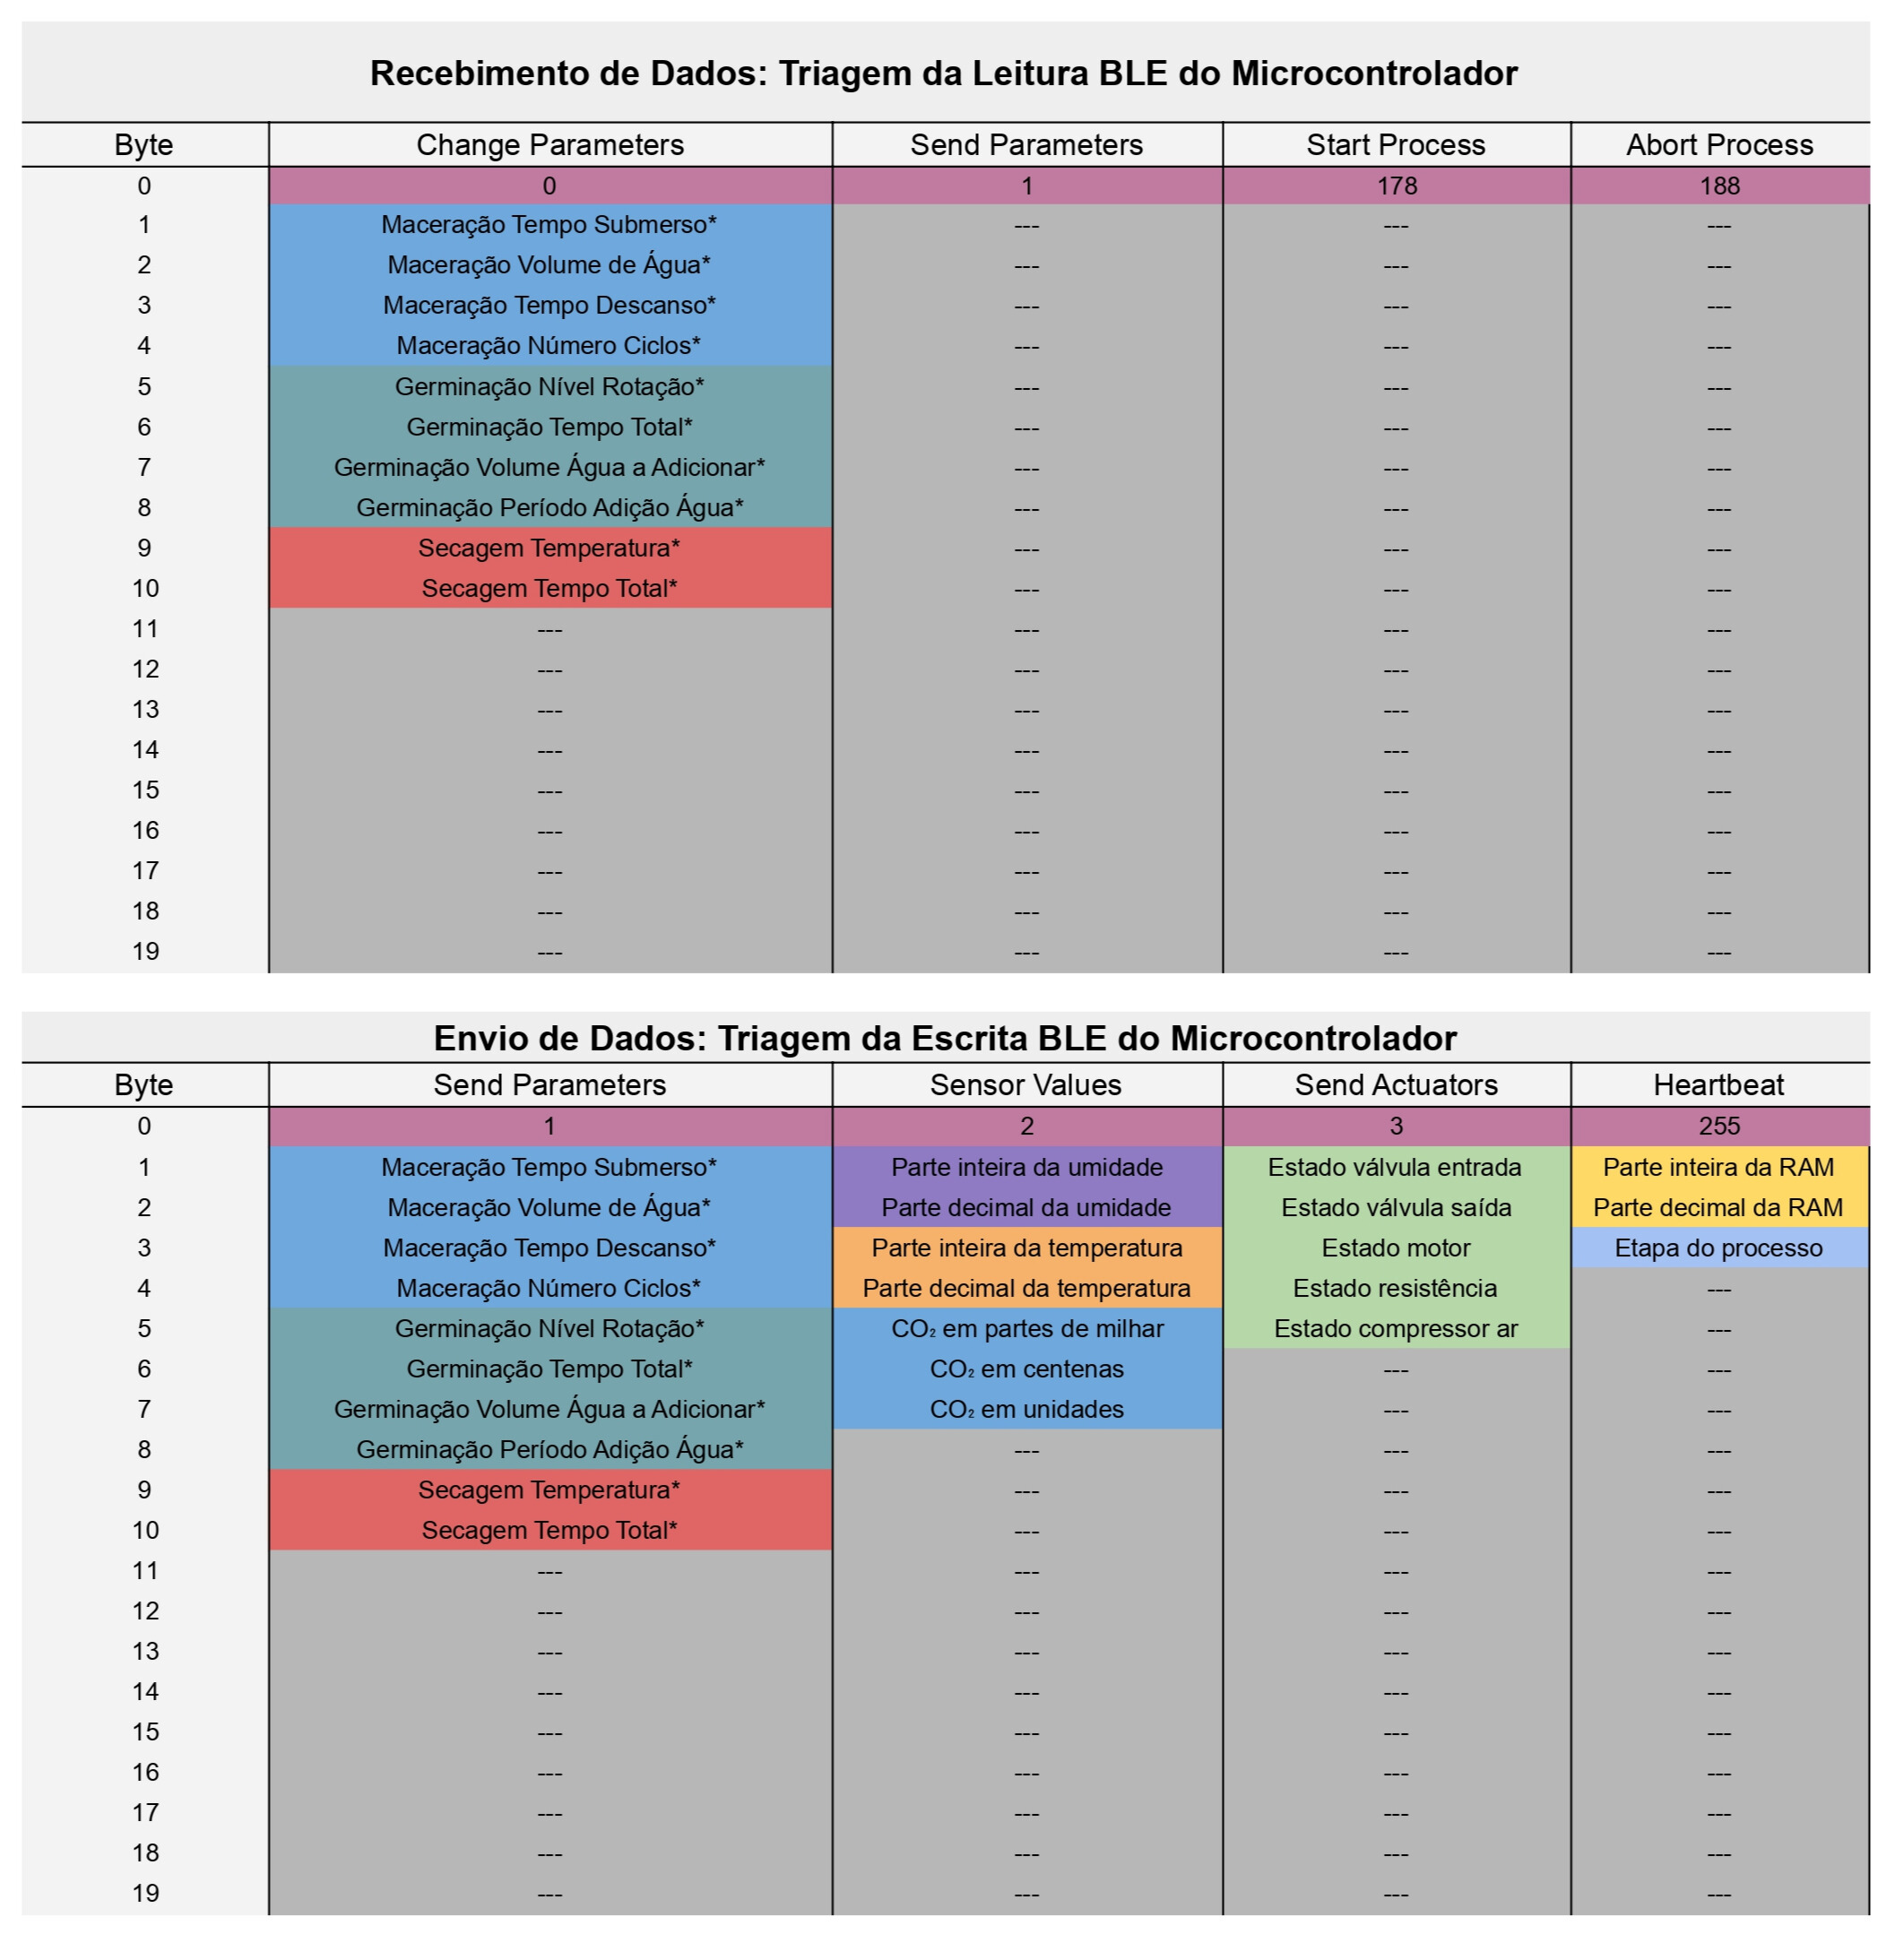
\includegraphics[width=1.0\textwidth]{Tabela-bytes.png}

    {\centering\footnotesize Fonte: Autoria própria.\par}
\end{figure}

Para exemplificar, na função de envio do \textit{heartbeat}, a variável \texttt{message}, em que se constrói o pacote a ser enviado, representa um \textit{array} construído por meio da classe \texttt{WriteList}, de onde é extraído o identificador correspondente. Este identificador é utilizado no aplicativo receptor para direcionar o tratamento da mensagem, garantindo a correta interpretação dos dados enviados.

\begin{figure}[H]
\lstinputlisting[
    language=Python,
    caption=Definição de constantes de identifação de pacote,
    label={lst:classreadlist}
    ]{algoritmos/classreadlist.py}
\end{figure}   

A lógica de comunicação implementada no aplicativo Android segue o mesmo princípio de identificação adotado no firmware. O primeiro byte do pacote recebido é utilizado como identificador, sendo interpretado para direcionar o tratamento adequado dos dados. Por exemplo, quando esse identificador assume o valor 255, entende-se que o pacote refere-se ao sinal de \textit{heartbeat} enviado periodicamente pelo ESP32, contendo também o percentual de uso da memória RAM e o estado atual do processo codificado.

Nesse contexto, o aplicativo interpreta os bytes seguintes como valores numéricos que representam, respectivamente, a parte inteira e a parte decimal da porcentagem. Esses valores são somados após a conversão para o formato numérico adequado, resultando em um valor final com duas casas decimais. Esse número é então utilizado para atualizar a interface do usuário com a informação atualizada sobre o consumo de memória do dispositivo.

Além da extração dos dados de uso de memória, o recebimento do identificador 255 também aciona uma função interna responsável por sinalizar a chegada do \textit{heartbeat}. Esse mecanismo funciona como um pulso periódico enviado pelo firmware, cuja função principal é indicar que o dispositivo segue ativo e em comunicação com o aplicativo. No aplicativo, esse pulso ativa um recurso visual na interface: uma indicação em forma de círculo que pisca a cada novo recebimento. Esse indicador atua como um monitor de conexão em tempo real, permitindo ao usuário verificar de forma intuitiva se a comunicação Bluetooth está estável. Caso o pulso deixe de ser recebido por um intervalo prolongado, o usuário deve observar que ocorreu a perda de sinal ou falha de comunicação, evitando a falsa impressão de que o sistema permanece operacional quando, na verdade, pode estar congelado ou desconectado.

Esse modelo de tratamento baseado em identificadores garante clareza na separação das funções e facilita futuras expansões, mantendo o código modular e de fácil manutenção.


\subsection{Parâmetros de malteação}

Os parâmetros de malteação correspondem às variáveis de controle utilizadas para configurar e ajustar o processo, como tempos de etapa, temperatura alvo e outros valores relevantes. Esses dados são essenciais para garantir a execução correta das etapas automatizadas.

Durante a inicialização do sistema, o firmware realiza a leitura de um arquivo de configuração persistente, armazenado localmente na memória do ESP32. Esse arquivo, no formato JSON, contém os valores salvos da última configuração utilizada. O conteúdo lido é mapeado internamente para as variáveis de controle do sistema, tornando-as acessíveis para os demais módulos do firmware.

Além da leitura, o sistema também permite a atualização desses parâmetros via comunicação Bluetooth. Sempre que o aplicativo envia novos valores, eles são armazenados temporariamente, validados e, posteriormente, gravados no arquivo de configuração. Isso garante que as alterações permaneçam ativas mesmo após desligamentos ou reinicializações.

A lógica geral de carregamento e persistência dos parâmetros é representada na \autoref{fig:fluxoparametros}, que ilustra o fluxo completo de inicialização e atualização dos dados operacionais do malteador.

\begin{figure}[H]
    \centering
    \caption{Fluxo de inicialização e atualização dos parâmetros de malteação.}
    \label{fig:fluxoparametros}
    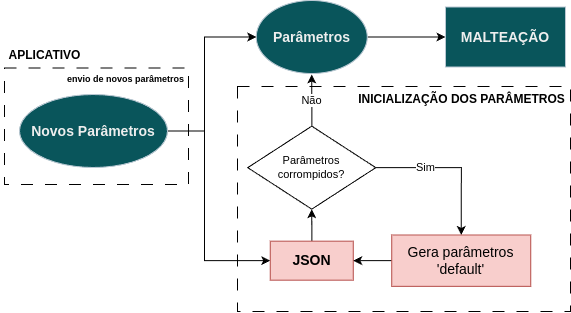
\includegraphics[width=0.9\textwidth]{fluxoparametros.png}

    {\centering\footnotesize Fonte: Autoria própria.\par}
\end{figure}

Os parâmetros de malteação foram otimizados para que seus valores pudessem ser representados dentro da faixa de um único byte, permitindo até 256 variações distintas por parâmetro. Essa decisão buscou equilibrar a precisão necessária para o controle do processo com a eficiência na comunicação via Bluetooth, já que o envio de todos os parâmetros em um único pacote reduz o tempo de transmissão e minimiza o risco de perda de pacotes.

Embora essa abordagem limite a resolução de cada parâmetro, ela se mostra adequada frente às grandezas envolvidas no processo. Caso, em futuras otimizações, identifique-se a necessidade de representar valores com maior precisão, a arquitetura atual do sistema permite a adição de bytes extras sem impactos significativos na estrutura dos módulos.

A conversão dos valores numéricos para um único byte é feita por meio de uma transformação linear, na qual o valor transmitido (inteiro entre 0 e 255) é multiplicado por um fator de escala e somado a um valor mínimo admissível. Esse procedimento garante que a representação final esteja sempre dentro da faixa operacional válida para cada variável.

As Tabelas~\ref{tab:coefmac}, \ref{tab:coefgerm} e \ref{tab:coefsec} apresentam os coeficientes utilizados para a reconstrução dos valores reais a partir dos dados recebidos via Bluetooth. Para cada parâmetro, aplica-se a seguinte fórmula:

\begin{center}
    \textit{valor real} = (\textit{byte recebido} × MULT\_TEN) + MIN\_VALUE
\end{center}

Esse mesmo modelo é utilizado na conversão inversa, durante a serialização dos dados antes da transmissão, garantindo consistência entre os módulos do firmware e do aplicativo.

\begin{table}[H]
    \caption{Coeficientes de reconstrução — Etapa de Maceração}
    \label{tab:coefmac}
    \centering
    \begin{tabular}{lcc}
        \hline
        \bfseries Parâmetro & \bfseries MULT\_TEN & \bfseries MIN\_VALUE \\
        \hline
        Tempo Submerso     & 1.0  & 1.0   \\
        Volume de Água     & 10.0 & 200.0 \\
        Tempo de Descanso  & 0.1  & 0.0   \\
        Número de Ciclos   & 1.0  & 1.0   \\
        \hline
    \end{tabular}
    
    {\centering\footnotesize Fonte: Autoria própria.\par}
\end{table}

\begin{table}[H]
    \caption{Coeficientes de reconstrução — Etapa de Germinação}
    \label{tab:coefgerm}
    \centering
    \begin{tabular}{lcc}
        \hline
        \bfseries Parâmetro & \bfseries MULT\_TEN & \bfseries MIN\_VALUE \\
        \hline
        Nível de Rotação    & 1.0 & 0.0  \\
        Tempo Total         & 1.0 & 24.0 \\
        Volume de Água      & 1.0 & 100.0 \\
        Adição de Água      & 1.0 & 10.0 \\
        \hline
    \end{tabular}
    
    {\centering\footnotesize Fonte: Autoria própria.\par}
\end{table}

\begin{table}[H]
    \caption{Coeficientes de reconstrução — Etapa de Secagem}
    \label{tab:coefsec}
    \centering
    \begin{tabular}{lcc}
        \hline
        \bfseries Parâmetro & \bfseries MULT\_TEN & \bfseries MIN\_VALUE \\
        \hline
        Temperatura  & 1.0 & 40.0 \\
        Tempo Total  & 0.1 & 1.0  \\
        \hline
    \end{tabular}
    
    {\centering\footnotesize Fonte: Autoria própria.\par}
\end{table}

Na \autoref{tab:parametros}, são listados todos os parâmetros disponíveis no sistema, acompanhados de suas respectivas faixas de valores operacionais, definidas conforme os limites estabelecidos.

\begin{table}[H]
    \caption{Faixa de valores possíveis para cada parâmetro.}
    \label{tab:parametros}
    \centering
    \begin{tabular}{cccc}
        \hline
        \bfseries Parâmetro & \bfseries Etapa & \bfseries Faixa de Valores & \bfseries Unidade \\
        \hline
        Tempo Submerso & Maceração & 1 -- 256  & horas \\
        Volume de Água & Maceração & 200 -- 2750 & mL \\
        Tempo de Descanso & Maceração & 0.0 -- 25,5 & horas \\
        Número de Ciclos & Maceração & 1 -- 256 & ciclos \\
        Nível de Rotação & Germinação & 0 -- 255 & -- \\
        Tempo Total & Germinação & 24 -- 279 & horas \\
        Volume de Água & Germinação & 100 -- 355 & mL \\
        Adição de Água & Germinação & 10 -- 265 & minutos \\
        Temperatura & Secagem & 40 -- 295 & $^{\circ}$C \\
        Tempo Total & Secagem & 1.0 -- 26.5 & horas \\
        \hline
    \end{tabular}

    {\centering\footnotesize Fonte: Autoria própria.\par}
\end{table}



\subsection{Algoritmo da malteação}

O controle automatizado da malteação foi implementado com base em uma lógica assíncrona, permitindo a execução simultânea de múltiplas tarefas relacionadas ao processo. A arquitetura do algoritmo principal é centrada em um sistema de estados, no qual cada etapa do processo (maceração, germinação e secagem) é tratada como um estágio independente, com mecanismos de inicialização, monitoramento e interrupção.

A execução do processo é iniciada a partir de um comando enviado pelo aplicativo, o que ativa a função responsável pela coordenação da malteação. Essa função inicializa o estado global e delega a execução para funções específicas de cada etapa, que operam com base nas configurações previamente definidas (parâmetros).

Durante toda a execução, o sistema monitora constantemente um sinal de interrupção, que pode ser acionado a qualquer momento via comunicação Bluetooth. Essa lógica garante que o processo possa ser encerrado de forma segura e imediata, sem comprometer a integridade das etapas já concluídas.

\subsubsection{Maceração}

A etapa de maceração é composta por dois fluxos assíncronos que atuam de forma paralela: o controle térmico, responsável por manter a temperatura adequada do sistema, e o controle de tempo, que regula a execução dos ciclos de hidratação.

Cada ciclo da maceração é formado por quatro subetapas executadas sequencialmente:

\begin{enumerate}
    \item \textbf{Enchimento}: o reservatório é preenchido com água até o volume desejado.
    \item \textbf{Imersão}: os grãos permanecem submersos pelo tempo programado.
    \item \textbf{Drenagem}: a água é escoada do sistema.
    \item \textbf{Repouso}: há uma pausa antes do próximo ciclo.
\end{enumerate}

Essas fases são repetidas conforme o número de ciclos configurado pelo usuário. A execução da etapa de maceração pode ser representada de forma resumida na Tabela~\ref{tab:maceracao-fluxo}.

\begin{table}[H]
    \caption{Fluxo de controle da etapa de maceração}
    \label{tab:maceracao-fluxo}
    \centering
    \begin{tabular}{>{\bfseries}c p{10cm}}
        \hline
        Fase & Descrição \\
        \hline
        Inicialização & Define o estado do sistema como \texttt{steeping}, carrega os parâmetros de ciclo e inicia tarefas assíncronas. \\
        Controle térmico & Mantém a temperatura dentro do intervalo alvo por meio de resfriamento ativo. Executado em paralelo. \\
        Controle de tempo & Executa a sequência de subetapas (enchimento, imersão, drenagem, repouso) para cada ciclo. \\
        Interrupção & A cada subetapa, o sistema verifica continuamente se houve solicitação de parada. \\
        Finalização & Ao término dos ciclos ou interrupção, o sistema atualiza o estado para inativo. \\
        \hline
    \end{tabular}
    
    {\centering\footnotesize Fonte: Autoria própria.\par}
\end{table}

O controle de válvulas, tanto para enchimento quanto para drenagem, segue um modelo baseado no tempo de abertura, adicionando o volume necessário para a operação. Apesar de simplificado, esse método pode ser ajustado posteriormente com base em calibrações que relacionem diretamente o tempo de válvula aberta ao volume de água processado. Esse aspecto é fundamental para permitir futuras melhorias sem a necessidade de reescrita da estrutura de controle.

A lógica de controle de temperatura foi implementada como uma tarefa paralela, executada em segundo plano com checagens periódicas e resposta imediata ao sinal de interrupção. Embora o protótipo atual ainda não possua capacidade física de controle térmico ativo (resfriamento), essa tarefa já está incorporada de forma modular no firmware, permitindo que sensores e atuadores possam ser integrados futuramente sem necessidade de grandes modificações estruturais. Essa abordagem garante escalabilidade e separação de responsabilidades, mantendo a coesão da arquitetura.

Ao final da execução dos ciclos de maceração, o sistema redefine o estado da etapa como inativo e passa automaticamente para o próximo estágio do processo, aguardando o início da germinação.

\subsubsection{Germinação}

A etapa de germinação (\textit{germination}) mantém a estrutura introduzida na maceração, com múltiplas tarefas assíncronas atuando de forma coordenada. Ao entrar nesse estágio, o sistema atualiza o estado global e ativa quatro tarefas principais, que operam em paralelo:

\begin{itemize}
    \item \textbf{Controle de tempo}: cronômetro responsável por definir a duração total da germinação.
    \item \textbf{Controle de temperatura}: ajusta ou monitora a temperatura ambiente.
    \item \textbf{Controle de umidade}: umidifica os grãos periodicamente.
    \item \textbf{Controle de rotação}: ativa mecanismos de movimentação dos grãos para arejamento.
\end{itemize}

Essas tarefas compartilham uma variável de sinalização comum, que permite a interrupção imediata da etapa caso o processo seja cancelado via aplicativo. A Tabela~\ref{tab:germinacao_fluxo} resume a lógica operacional da etapa de germinação.

\begin{table}[H]
    \caption{Fluxo de controle da etapa de germinação.}
    \label{tab:germinacao_fluxo}
    \centering
    \begin{tabular}{>{\bfseries}c p{10cm}}
        \hline
        Fase & Descrição \\
        \hline
        Inicialização & Atualiza o estado global para \texttt{germination} e carrega os parâmetros definidos. \\
        Controle temporal & Inicia o cronômetro principal da etapa. Ao fim do tempo total, sinaliza término da germinação. \\
        Controle ambiental & Controla e monitora temperatura e umidade em paralelo ao tempo. \\
        Controle de rotação & Aciona o sistema de movimentação dos grãos em intervalos regulares. \\
        Interrupção & Todas as tarefas verificam sinal de parada a cada ciclo. \\
        Finalização & Ao término do tempo ou interrupção, o sistema limpa o estado e prepara a etapa seguinte. \\
        \hline
    \end{tabular}

    {\centering\footnotesize Fonte: Autoria própria.\par}
\end{table}

A umidificação periódica dos grãos é feita por meio de ciclos de adição de água. O algoritmo alterna entre a abertura de válvulas para umidificar o ambiente e pausas programadas para não encharcar os grãos. Essa tarefa permanece ativa enquanto o estágio estiver em execução, repetindo os ciclos conforme o necessário. O controle de temperatura segue o mesmo princípio adotado na etapa anterior, sendo executado como tarefa independente que verifica periodicamente o estado do sistema, permitindo ajustes térmicos futuros.

O reservatório de água do protótipo foi planejado para suportar 5 litros, estima-se que este valor seja suficiente para o processo. Apesar disso, caso seja necessário, a implementação de um sensor de distância ultrassom para acompanhamento do nível do tanque será simples dada a arquitetura do firmware. 

Além disso, durante a germinação, o sistema realiza rotações constantes, para o revolvimento dos grãos com o objetivo de garantir a aeração e evitar o emaranhamento das radículas. Existe, também, leituras de CO$_{2}$ durante essa etapa para que seja possível emitir um alerta para o operador caso se atinja valores prejudiciais ao crescimento dos grãos.

\subsubsection{Secagem}

Encerrada a germinação, inicia-se a última etapa do processo: a secagem (\textit{kilning}). Nesta fase, o objetivo é reduzir a umidade dos grãos e interromper a atividade enzimática, preservando as características desejadas do malte. A lógica geral mantém o padrão assíncrono das etapas anteriores, com três tarefas paralelas operando de forma coordenada: controle de tempo, temperatura e rotação.

A Tabela~\ref{tab:secagem_fluxo} detalha o fluxo operacional da etapa de secagem:

\begin{table}[H]
    \caption{Fluxo de controle da etapa de secagem}
    \label{tab:secagem_fluxo}
    \centering
    \begin{tabular}{>{\bfseries}c p{10cm}}
        \hline
        Fase & Descrição \\
        \hline
        Inicialização & Atualiza o estado global para \texttt{kilning} \\
        Controle temporal & Gerencia a duração total do estágio através de contagem regressiva baseada nos parâmetros \\
        Controle térmico & Mantém temperatura elevada, utilizando ciclos de aquecimento e monitoramento contínuo \\
        Controle de rotação & Ativa mecanismos de revolvimento em intervalos programados para homogeneização \\
        Interrupção & Verificação contínua de sinal de parada durante todas as subetapas \\
        Finalização & Desativa sistemas térmicos e mecânicos, atualiza estado para inativo \\
        \hline
    \end{tabular}

    {\centering\footnotesize Fonte: Autoria própria.\par}
\end{table}

O controle de tempo define a duração total do estágio, monitorando continuamente a contagem regressiva com base nos parâmetros definidos pelo usuário. Já a temperatura, nesse estágio, assume papel ainda mais crítico, visto que a secagem envolve temperaturas elevadas e potencialmente danosas ao produto se não forem adequadamente controladas.

Por fim, o controle de rotação continua presente, com o intuito de garantir a homogeneidade da secagem e evitar a formação de zonas com retenção de umidade. Essa movimentação periódica dos grãos deve assegurar uma secagem eficiente e uniforme.

A estrutura assíncrona aplicada em todas as etapas da malteação permite ao sistema operar com múltiplos controles simultâneos, com segurança, responsividade e flexibilidade. A separação lógica das funções facilita tanto a manutenção do código quanto a sua expansão, criando uma base para futuras implementações automatizadas, como a inclusão de um programa de torra.
 
\subsection{Sensores e Atuadores}

Nesta implementação, foram utilizados dois sensores, ambos com arquitetura baseada no protocolo I\textsuperscript{2}C responsáveis pela aquisição de dados para o processo:

\begin{table}[H]
    \caption{Especificação dos sensores}
    \label{tab:sensores_atuadores}
    \centering
    \begin{tabular}{llp{8cm}}
        \hline
        \textbf{Sensor} & \textbf{Parâmetros} & \textbf{Função no processo} \\
        \hline
        AH20 & Temperatura e umidade relativa & Monitoramento contínuo das condições ambientais durante todas as etapas da malteação \\
        ENS160 & eCO\textsubscript{2} (equivalente de CO\textsubscript{2}) & Detecção e monitoramento da atividade metabólica dos grãos na fase de germinação \\
        \hline
    \end{tabular}
    
    {\centering\footnotesize Fonte: Autoria própria.\par}
\end{table}

A leitura dos sensores ocorre de maneira contínua e assíncrona na tarefa \texttt{sensors\_task}, garantindo atualização constante dos dados. Após cada leitura, os valores de temperatura, umidade e eCO\textsubscript{2} são armazenados em variáveis globais, facilitando o acesso por outras tarefas do sistema. Para fins de transmissão Bluetooth, os valores são convertidos em bytes e enviados periodicamente para o aplicativo dentro dessa própria função.

O tratamento de falhas também foi considerado: caso a leitura de qualquer sensor falhe, o sistema atribui valor zero como padrão, garantindo que o fluxo da comunicação continue sem interrupções.

Em paralelo à leitura de sensores, o sistema também gerencia cinco atuadores principais: duas válvulas (entrada e saída de água), um motor de rotação, uma resistência térmica e uma bomba de ar. A lógica de controle desses dispositivos é encapsulada na classe \texttt{Actuator}, desenvolvida para simplificar a manipulação dos pinos GPIO e abstrair as diferenças de lógica de acionamento.

Cada atuador é instanciado em \texttt{actuators} com seu respectivo nome e número de pino, e armazenado em um dicionário global para facilitar o acesso dinâmico por outras partes do sistema. A classe disponibiliza métodos como \texttt{on()}, \texttt{off()} e \texttt{toggle()}, além de uma função de verificação de estado atual. Dessa forma, o acionamento de cada dispositivo torna-se simples, confiável e rastreável (via terminal).

Além do controle direto, foi implementada uma função de envio do estado atual dos atuadores via Bluetooth, permitindo que o aplicativo visualize, em tempo real, quais dispositivos estão ativos no momento.

\section{Aplicativo Android}\label{sec:aplicativo-android}

\subsection{Tela Inicial: Conexão}\label{subsec:conexao}
Ao inicializar o aplicativo, o usuário é direcionado à interface de conexão. Nesta tela, é exibido centralmente o status "Não conectado", acompanhado de um indicador de estado pulsante no canto superior direito, que alterna entre azul e cinza a cada segundo, quando conectado. A conexão com o dispositivo ESP32, previamente pareado via Bluetooth, é estabelecida mediante acionamento do botão "Conectar", conforme ilustrado na \autoref{fig:int-inicial}.

\begin{figure}[H]
    \caption{Interface inicial do aplicativo.}
    \label{fig:int-inicial}
    \centering
    \subfloat[Desconectado\label{fig:first-off}]{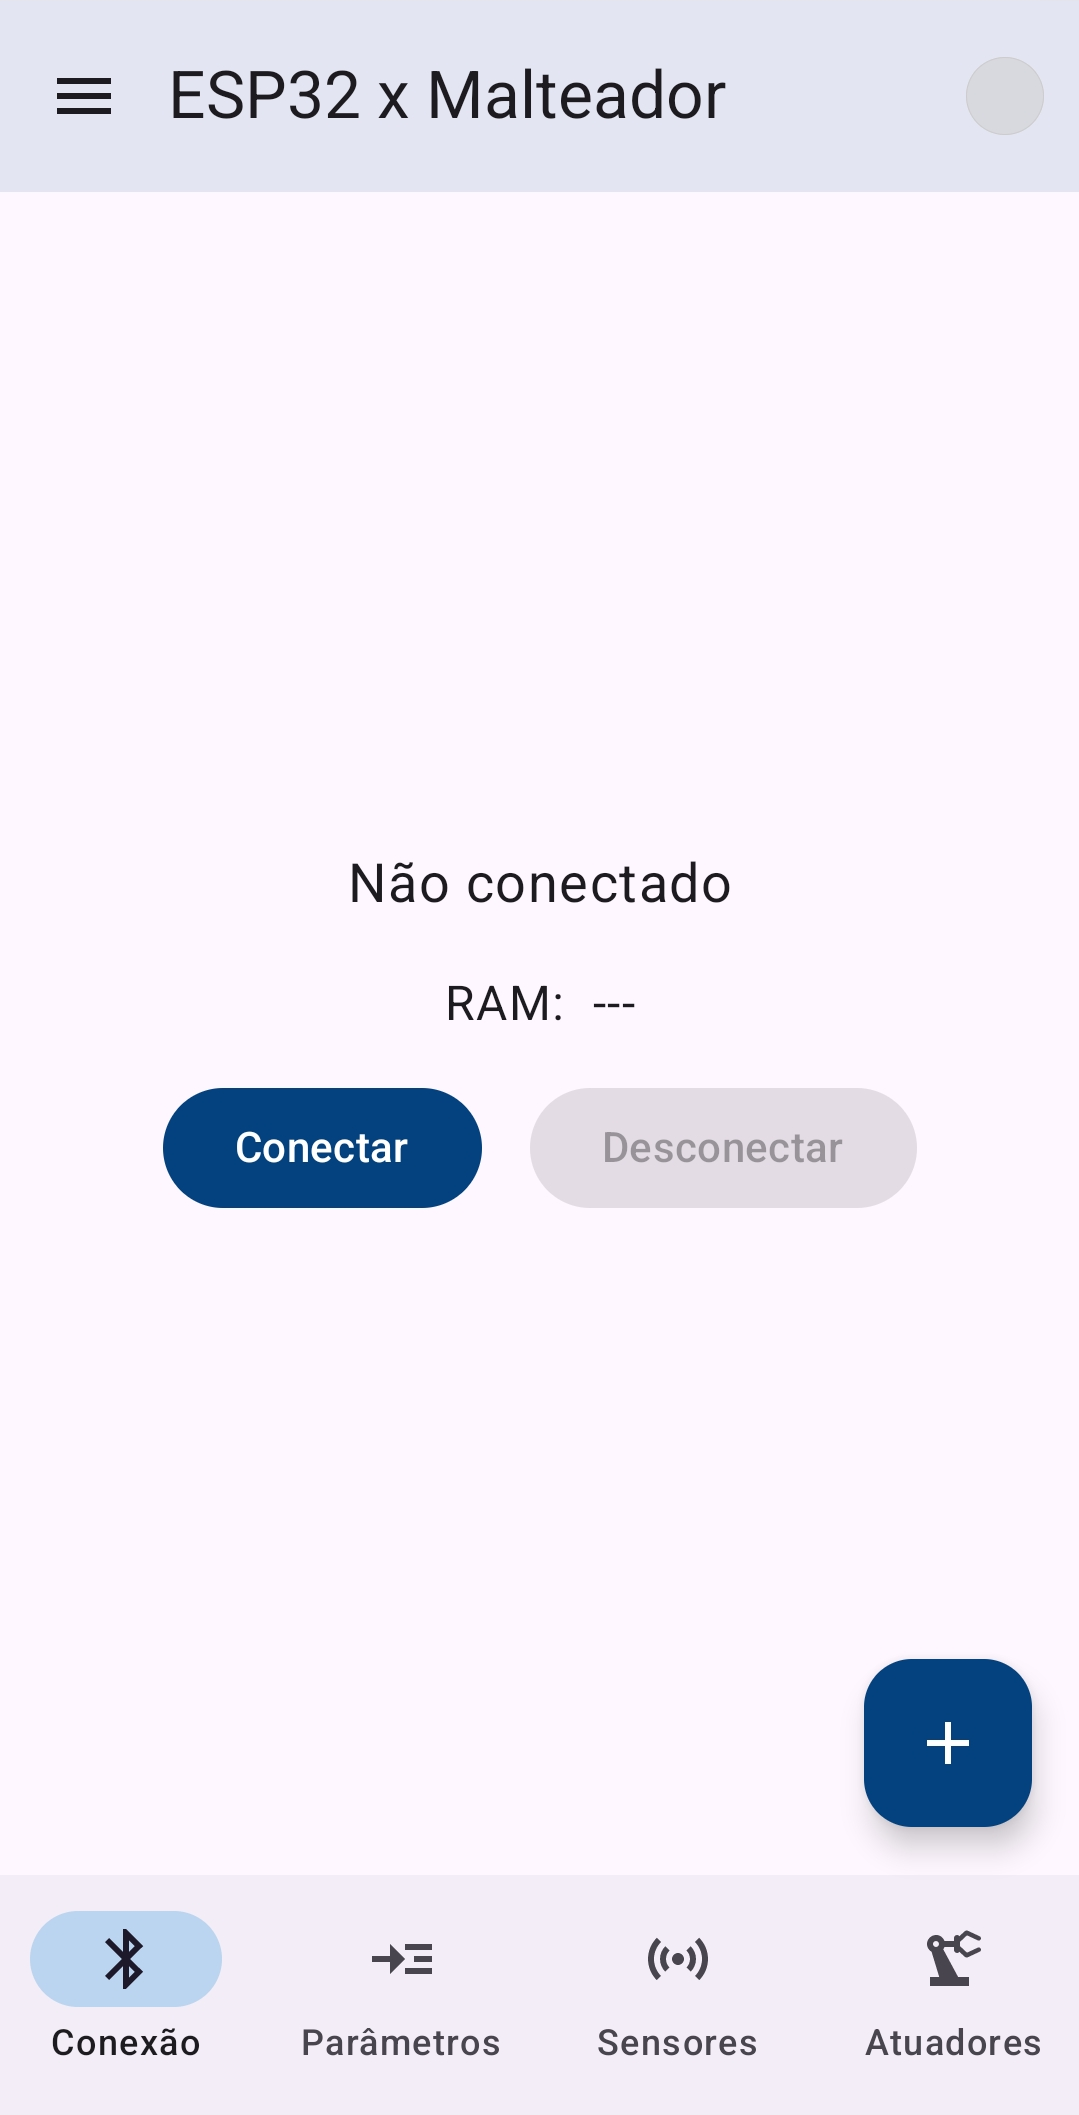
\includegraphics[width=0.3\textwidth]{first-off.png}}
    \hfill
    \subfloat[Conectado\label{fig:first-on}]{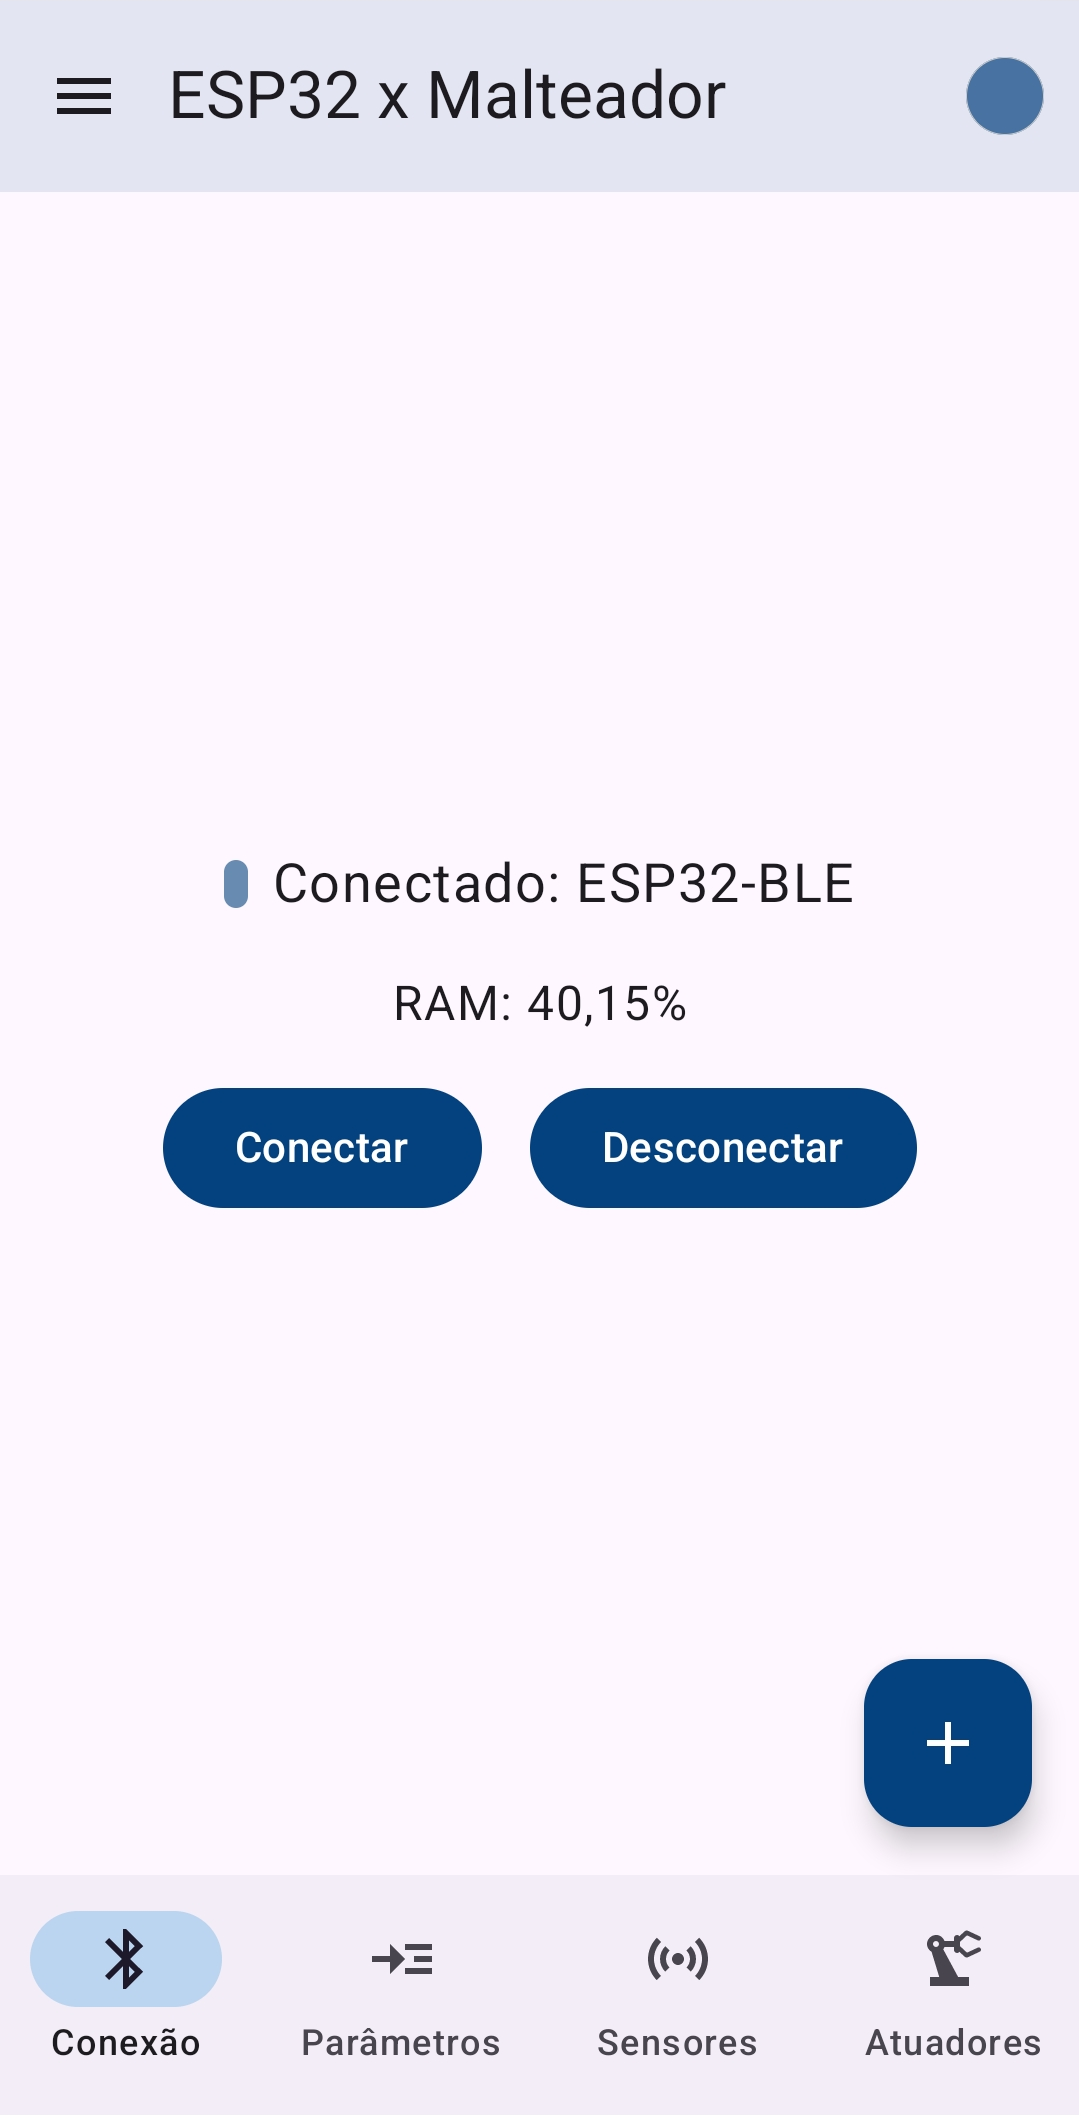
\includegraphics[width=0.3\textwidth]{first-on.png}}
    \hfill
    \subfloat[Tema escuro\label{fig:first-dark-theme}]{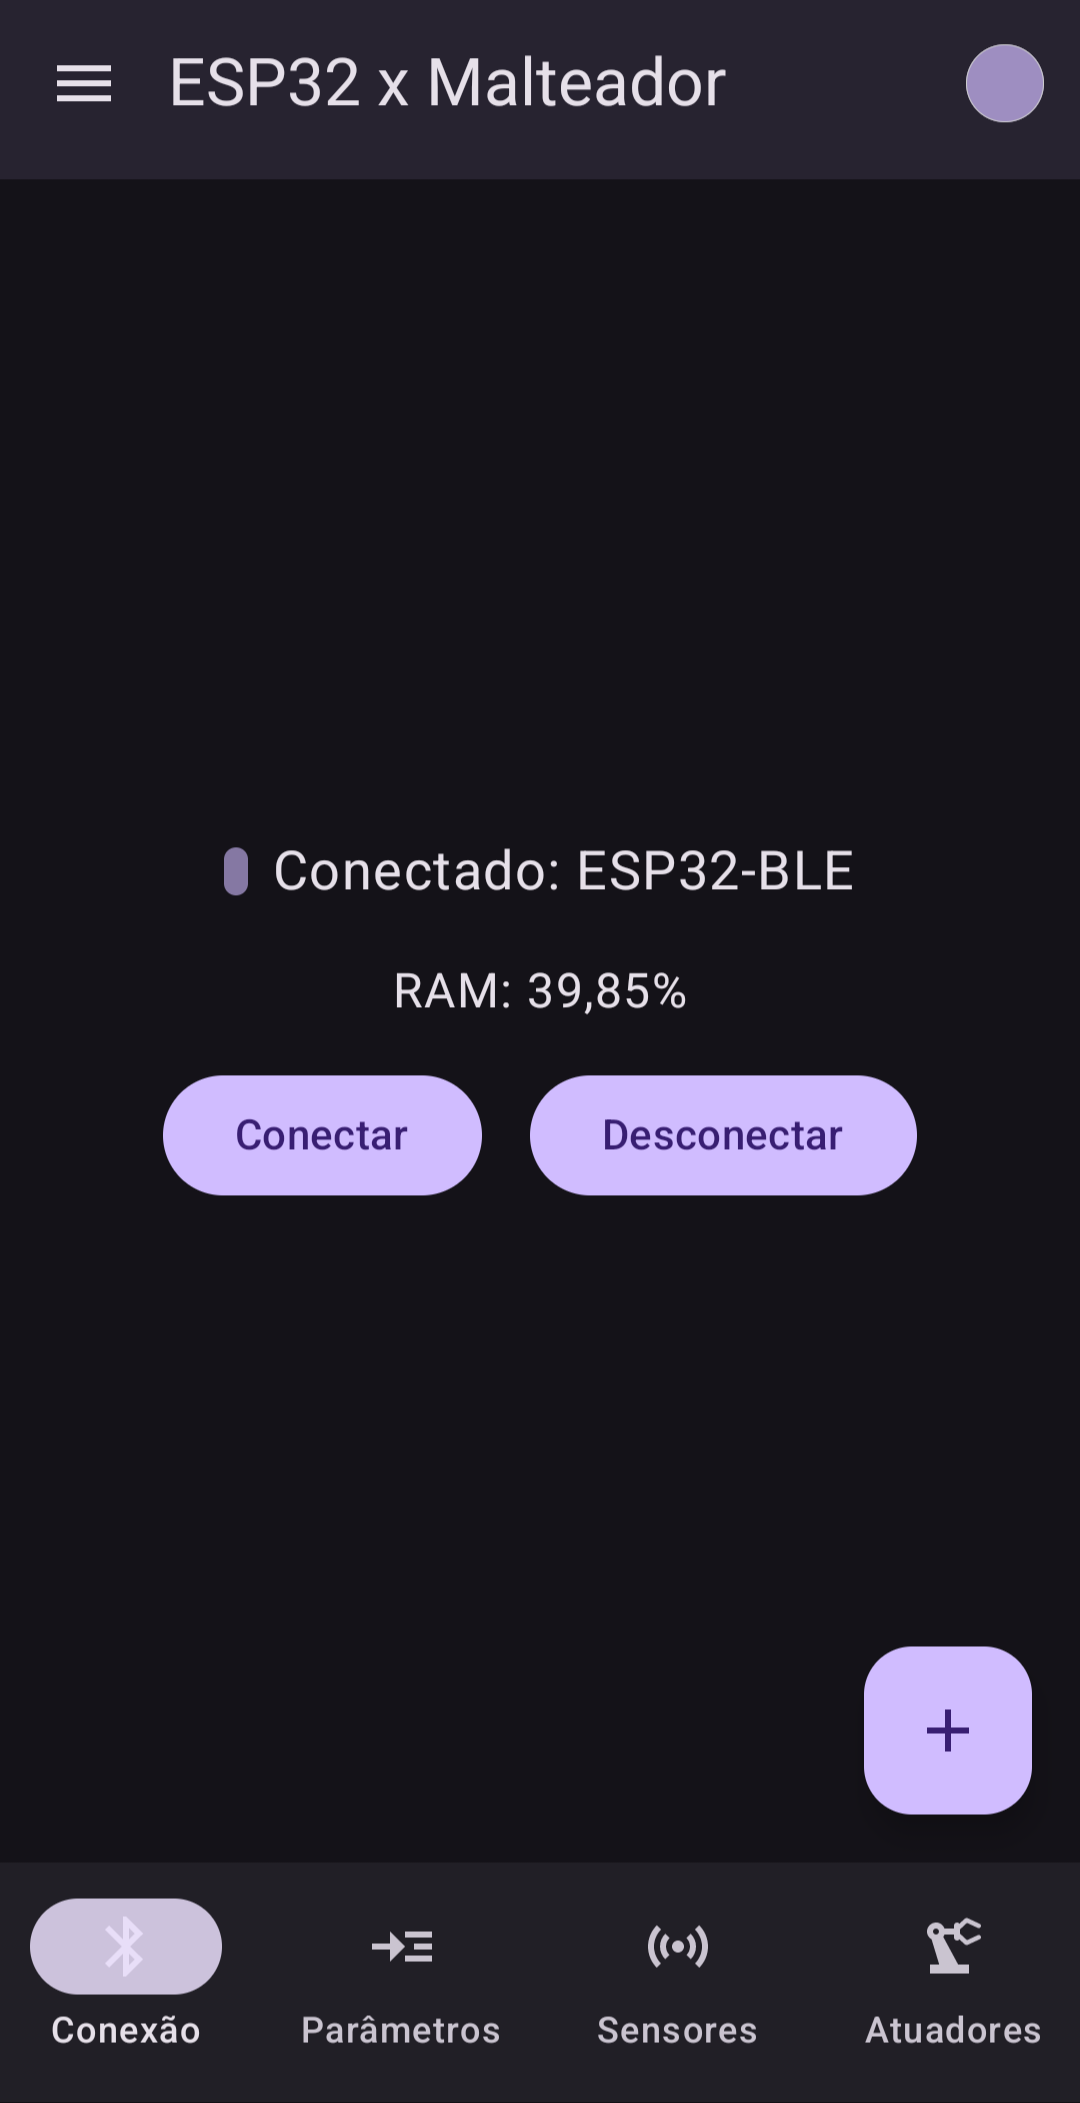
\includegraphics[width=0.3\textwidth]{first-dark-theme.png}}

    {\centering\footnotesize Fonte: Autoria própria.\par}

  \end{figure}


Ainda, na estrutura geral do \textit{Scaffold} (layout do aplicativo), destaca-se o \textit{FloatingActionButton} (FAB) no canto inferior direito. Este componente, ao ser acionado, expande um menu com funcionalidades essenciais, incluindo:

\begin{itemize}
    \item \textit{Verificar Parâmetros}, para sincronização dos parâmetros com o ESP32;
    \item \textit{Carregar Receita}, para autopreencher os parâmetros no aplicativo;
    \item \textit{Iniciar}, para enviar os parâmetros e iniciar o processo de malteação.
\end{itemize}

No canto superior esquerdo, o botão de navegação proporciona acesso ao \textit{Drawer}, um painel lateral com duas opções: "Início" (retorno à tela principal) e "Configurações" (\autoref{fig:drawer}). A tela de configurações, em sua versão atual, permite a alternância entre temas claro e escuro (\autoref{fig:int-inicial}), com previsão de expansão para personalizações avançadas, como definição de nomes de dispositivos e ajustes dos valores de UUID Bluetooth.

\begin{figure}[H]
    \caption{Drawer do aplicativo.}
    \label{fig:drawer}
    \centering
    \subfloat[Botão de acesso ao drawer\label{fig:DrawerButton}]{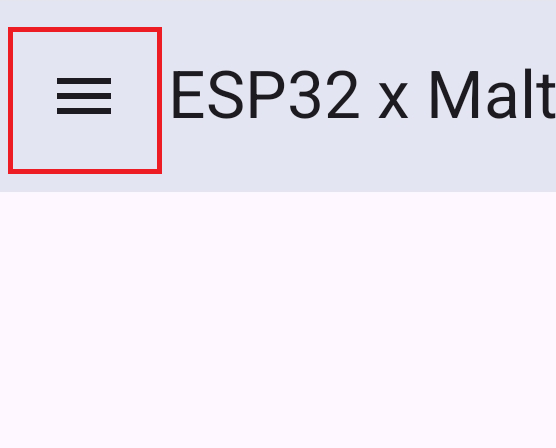
\includegraphics[width=0.3\textwidth]{DrawerButton.png}}
    \hfill
    \subfloat[Drawer aberto\label{fig:open-drawer}]{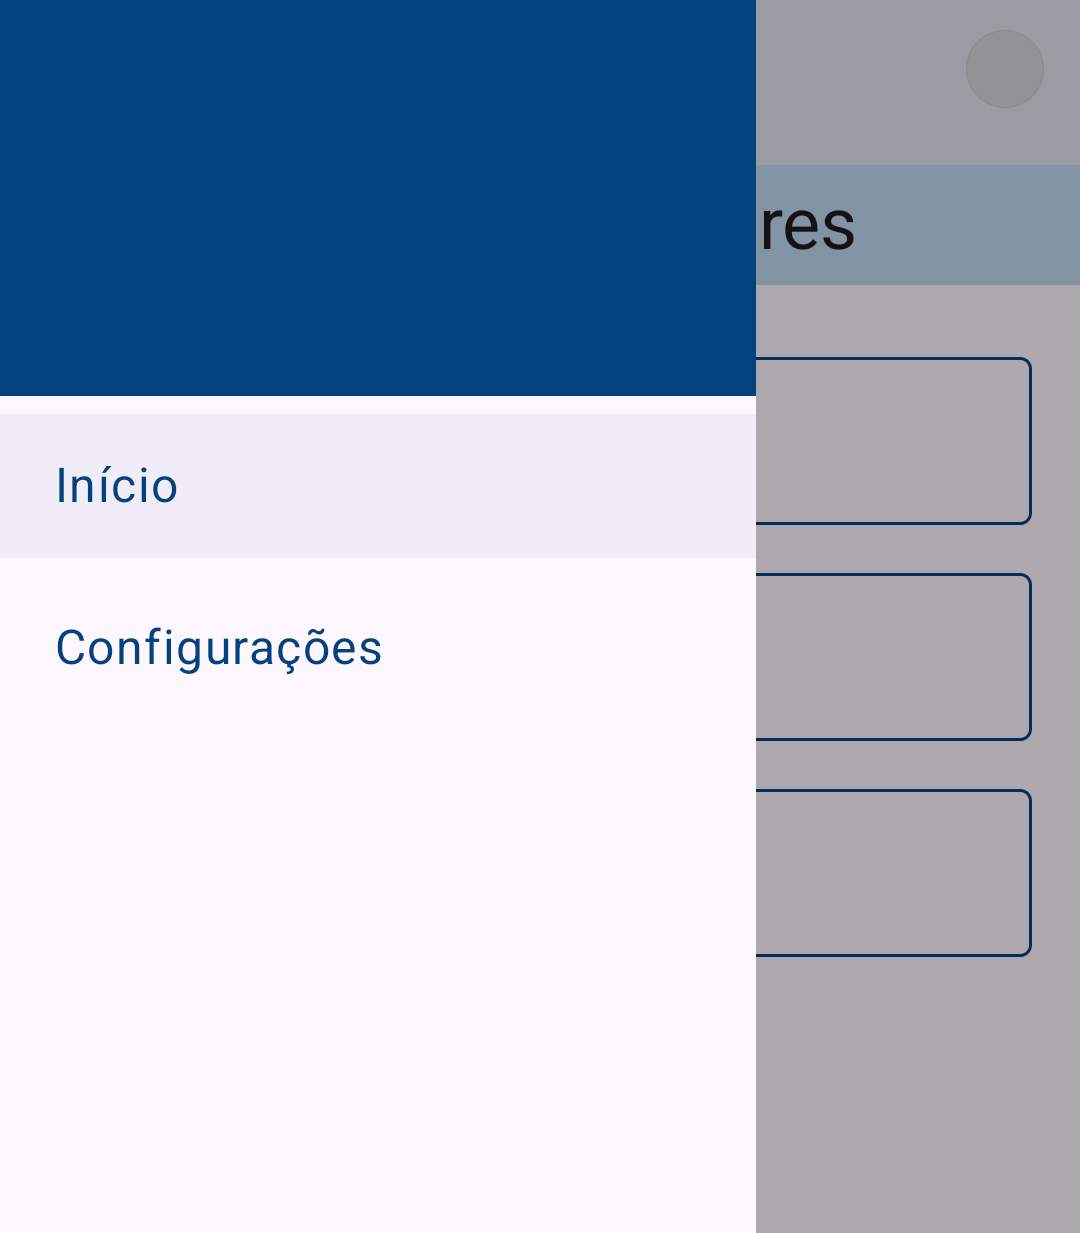
\includegraphics[width=0.3\textwidth]{open-drawer.png}}
    \hfill
    \subfloat[Tela de configurações acessada pelo drawer\label{fig:config-screen}]{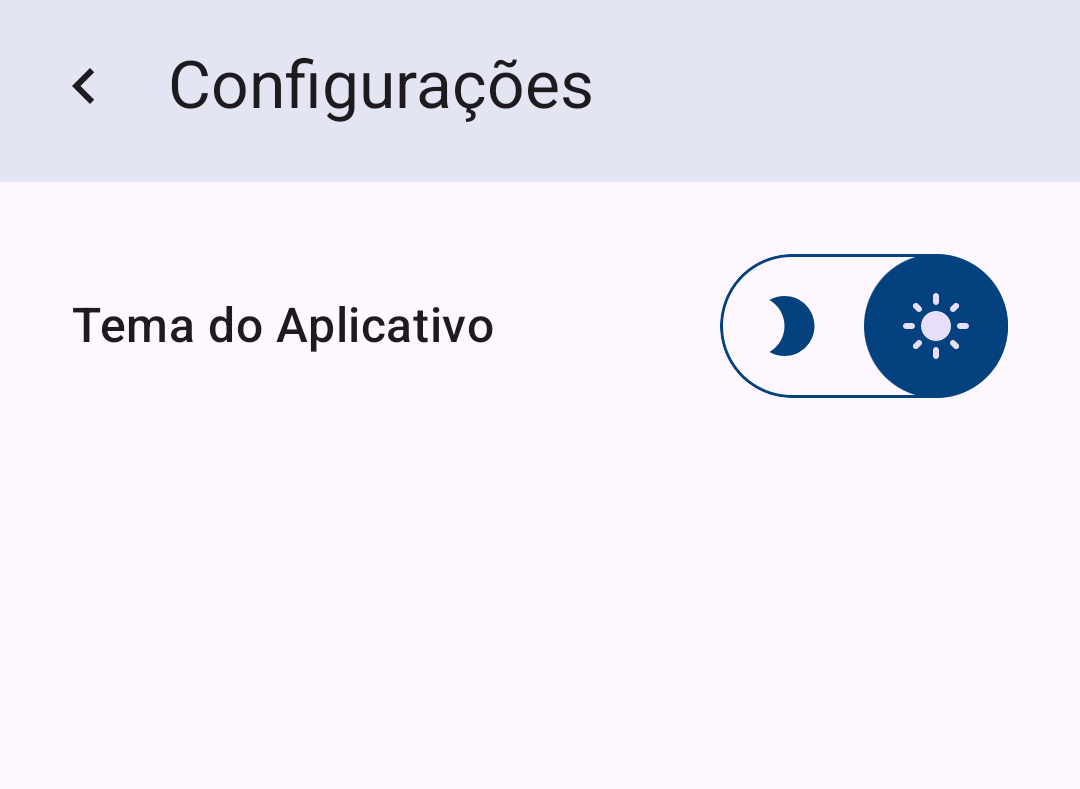
\includegraphics[width=0.3\textwidth]{config-screen.png}}

    {\centering\footnotesize Fonte: Autoria própria.\par}

  \end{figure}

\subsection{Tela de Parâmetros}\label{subsec:parametros}
A interface de parâmetros opera em dois modos distintos, conforme o estado de conexão. No modo desconectado (\autoref{fig:par-off}), os campos de entrada permanecem inativos. Quando conectado, os campos assumem codificação cromática dinâmica: tonalidade amarela para indicar valores não sincronizados ou nulos, e azul para valores válidos sincronizados com o ESP32 (\autoref{fig:parameters-state}). Valores fora da faixa operacional (\autoref{tab:parametros}) ou inconsistentes geram feedback visual impedindo o envio (\autoref{fig:parameters-state}), previnindo possíveis erros de extrapolação dos bytes na comunicação Bluetooth.

\begin{figure}[H]
    \centering
    \caption{Tela de parâmetros em modo desconectado com campos inativos.}
    \label{fig:par-off}
    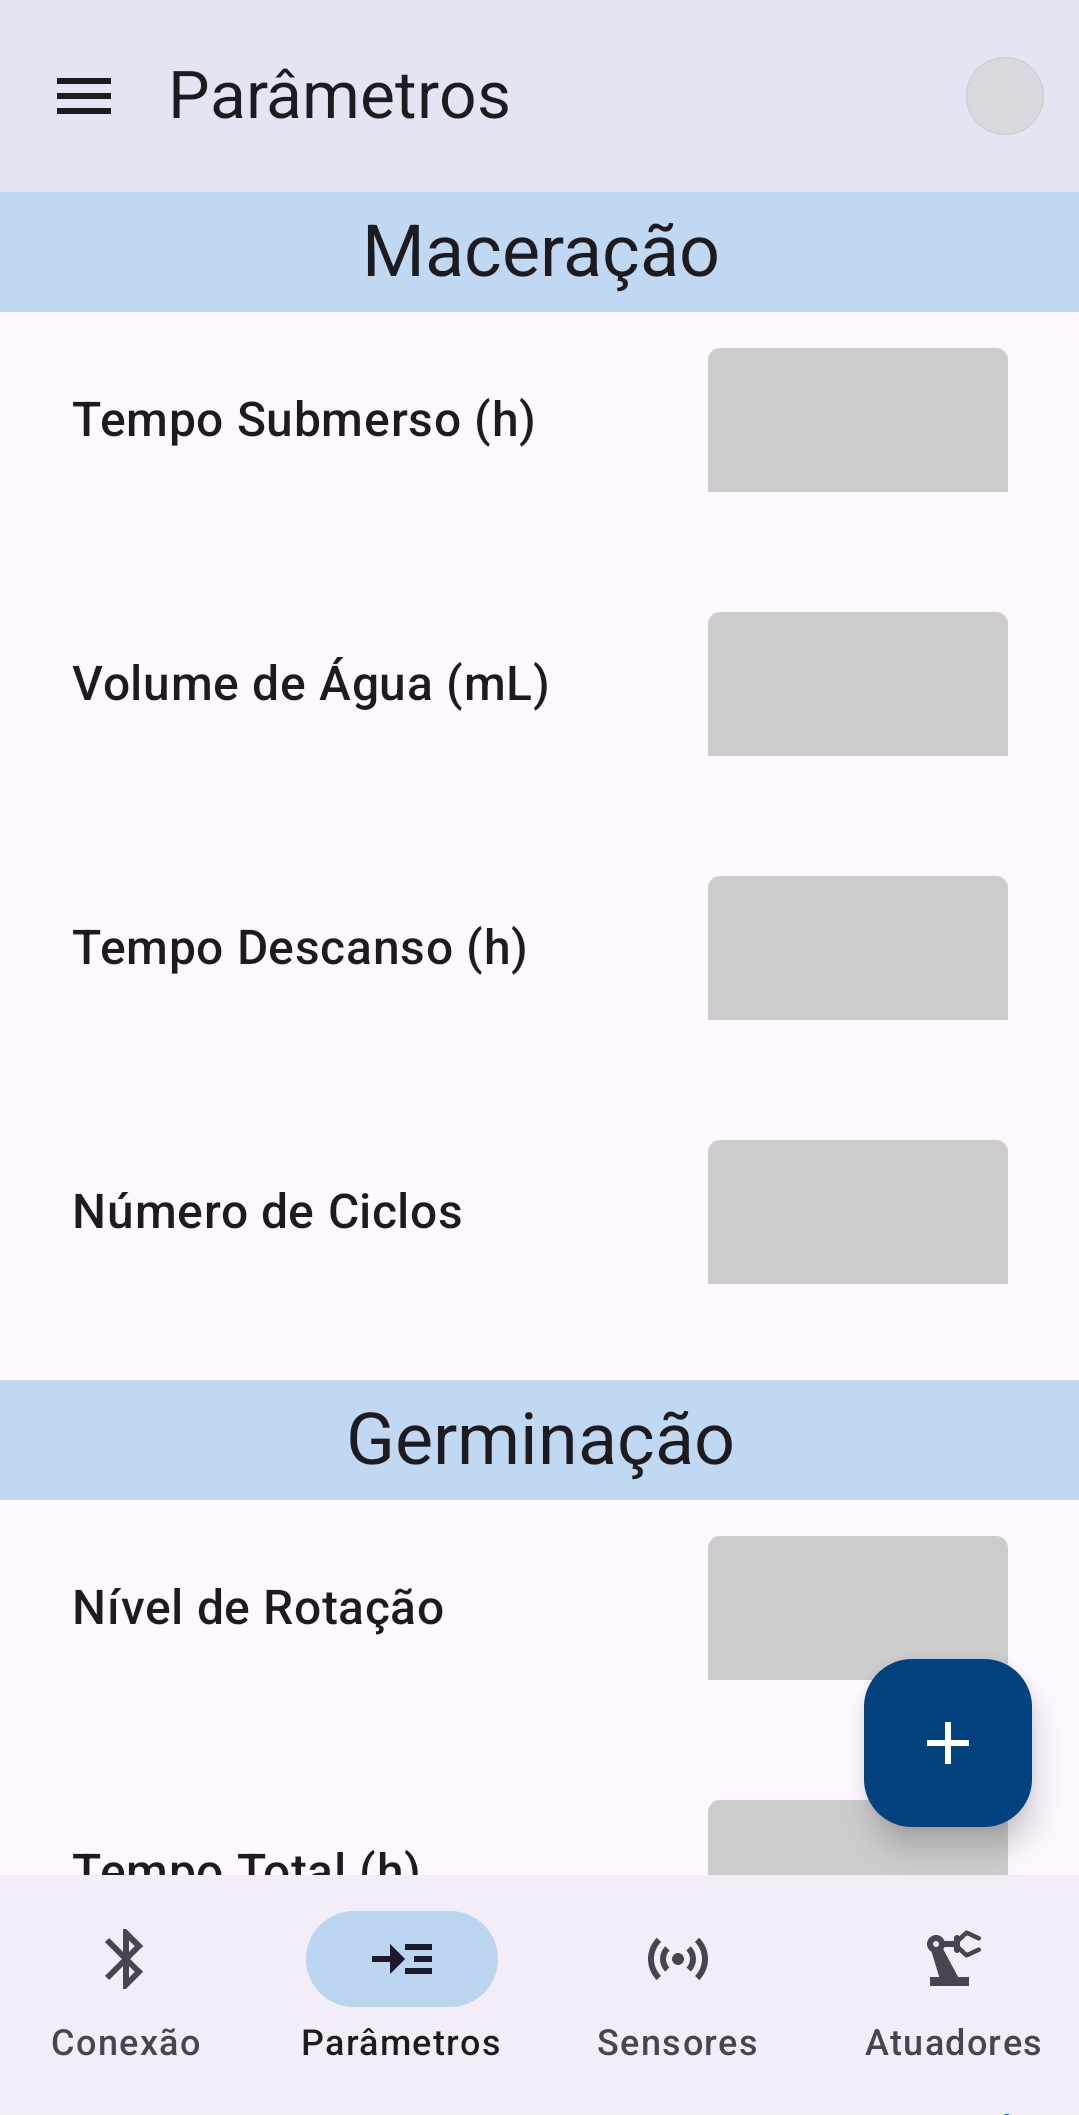
\includegraphics[width=0.32\textwidth]{par-off.png}

    {\centering\footnotesize Fonte: Autoria própria.\par}
\end{figure}

\begin{figure}[H]
    \caption{Estados dos campos de parâmetros.}
    \label{fig:parameters-state}
    \centering
    \subfloat[Campos de parâmetros em estado não sincronizado\label{fig:input-on-yellow}]{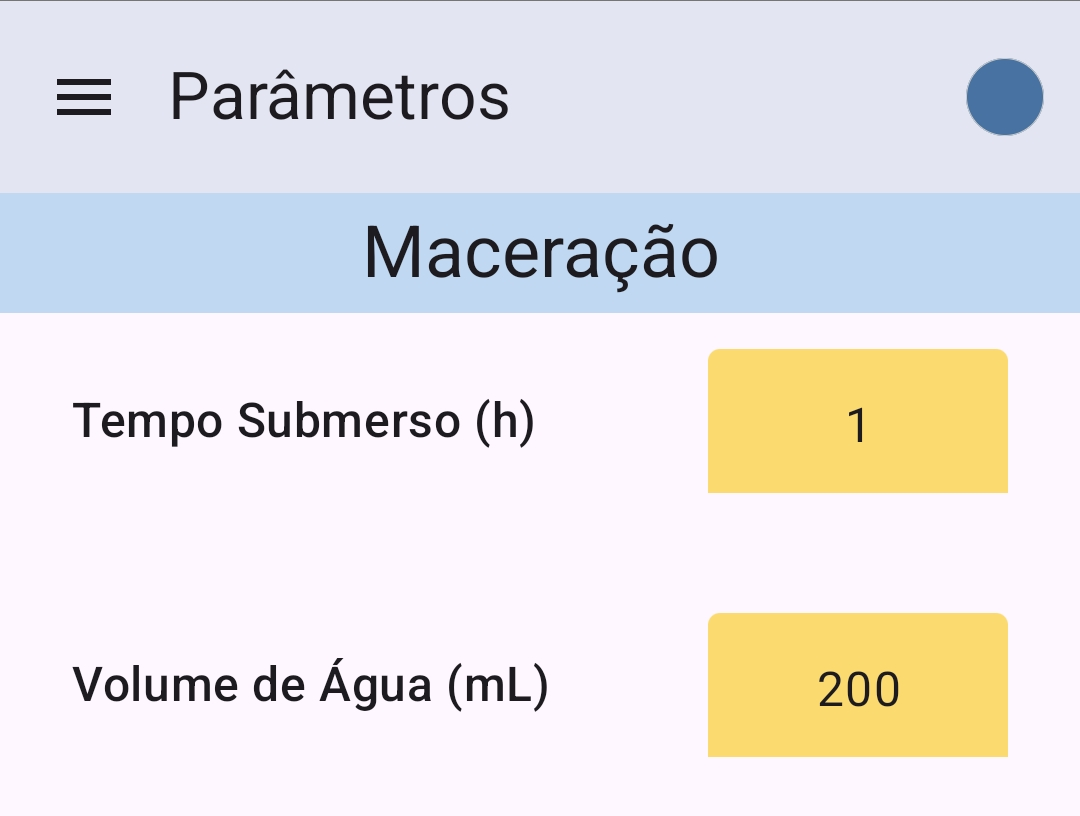
\includegraphics[width=0.4\textwidth]{input-on-yellow.png}}
    \hfill
    \subfloat[Campos de parâmetros válidos sincronizados\label{fig:input-on-blue}]{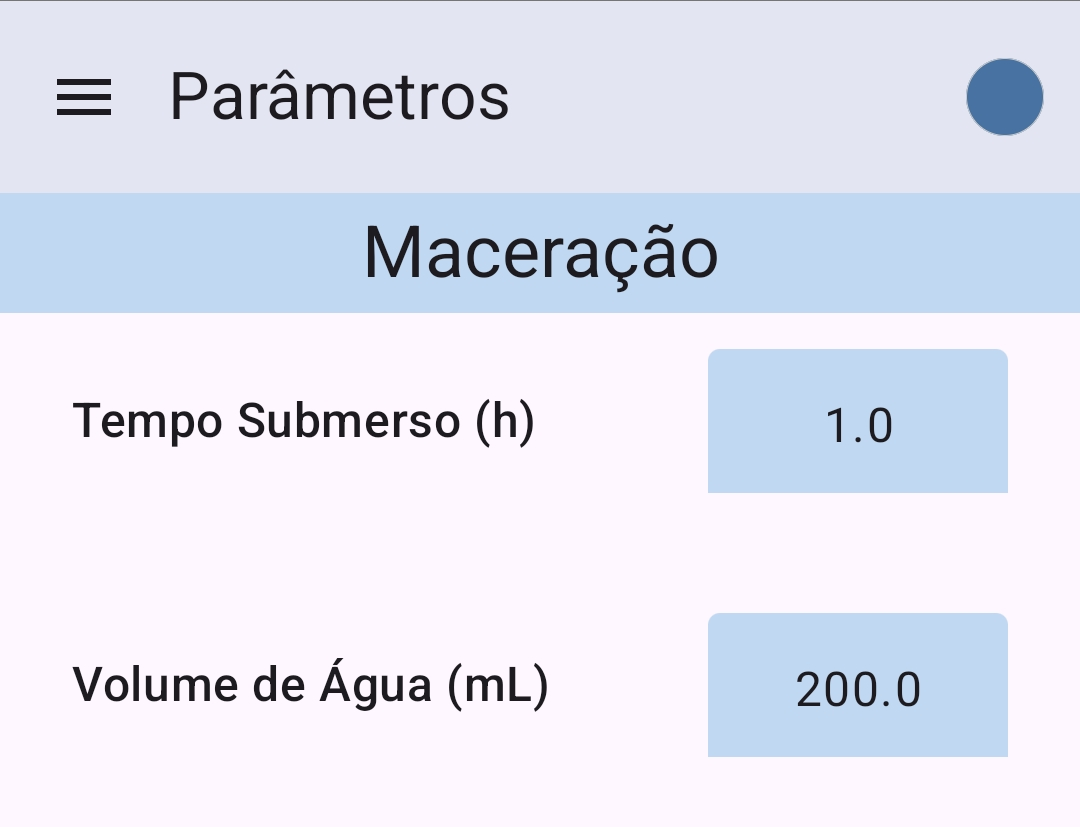
\includegraphics[width=0.4\textwidth]{input-on-blue.png}}
    \hfill
    \subfloat[Feedback visual para valores fora da faixa operacional\label{fig:out-range}]{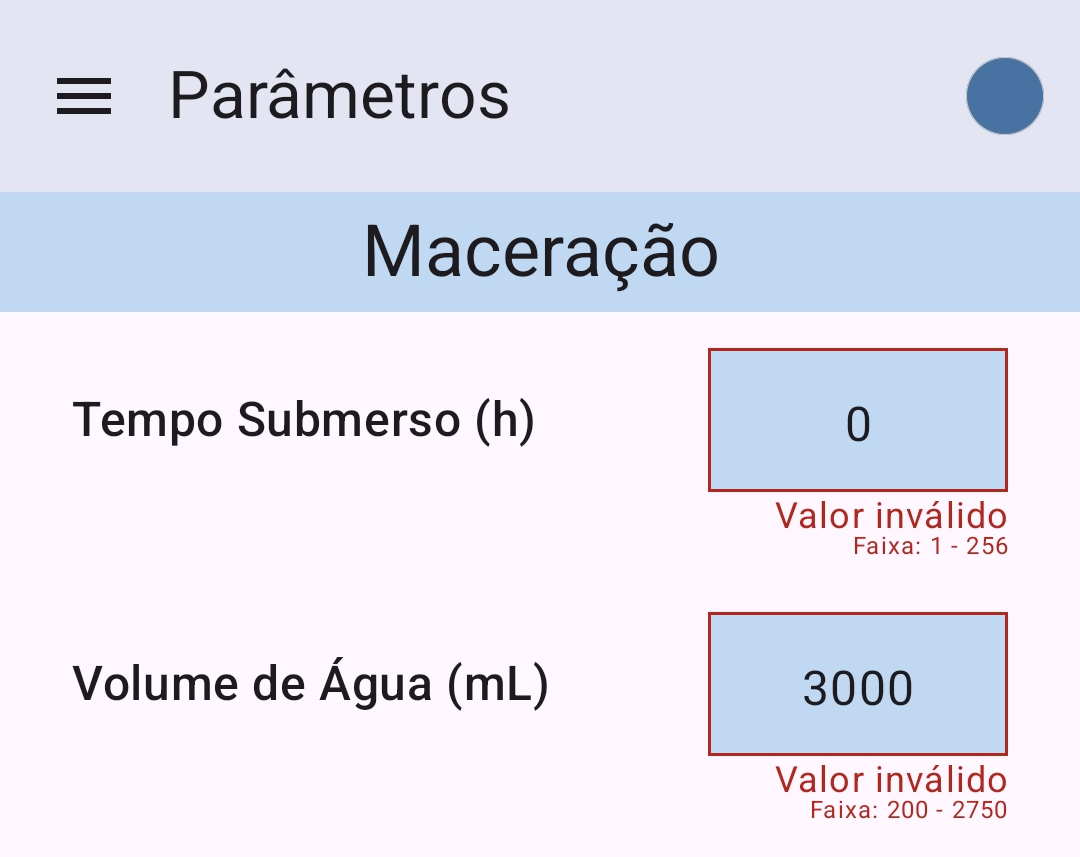
\includegraphics[width=0.4\textwidth]{out-range.png}}
    \hfill
    \subfloat[Feedback visual para valores nulos\label{fig:null-value}]{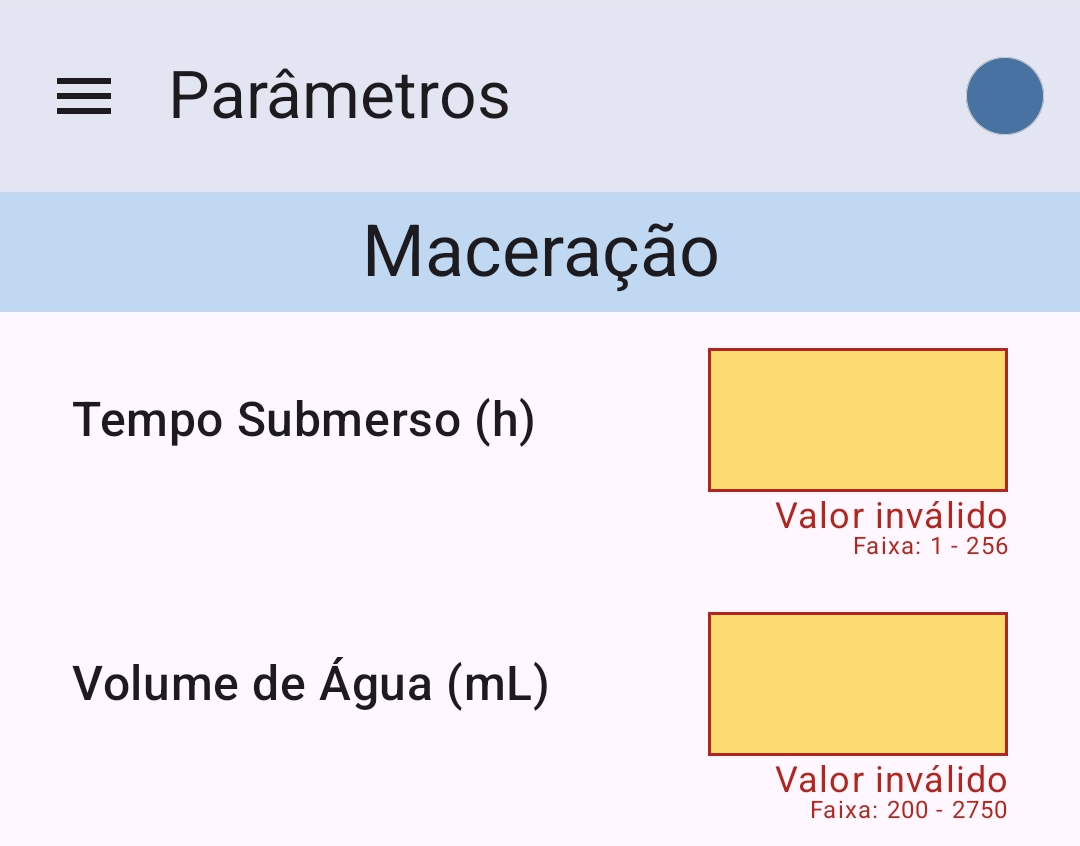
\includegraphics[width=0.4\textwidth]{null-value.png}}
    \hfill

    {\centering\footnotesize Fonte: Autoria própria.\par}

  \end{figure}


Para melhor experiência do usuário/operador, o sistema permite o armazenamento das configurações atuais de parâmetros como perfis personalizados ("receitas"), mediante nomeação em diálogo dedicado (\autoref{fig:select-save-recipe}). Essas receitas podem ser recuperadas através do menu do FAB, que exibe uma lista de opções salvas.

\begin{figure}[H]
    \caption{Salvamento e seleção de receitas}
    \label{fig:select-save-recipe}
    \centering
    \subfloat[Botão de salvamento de receitas\label{fig:save-recipe}]{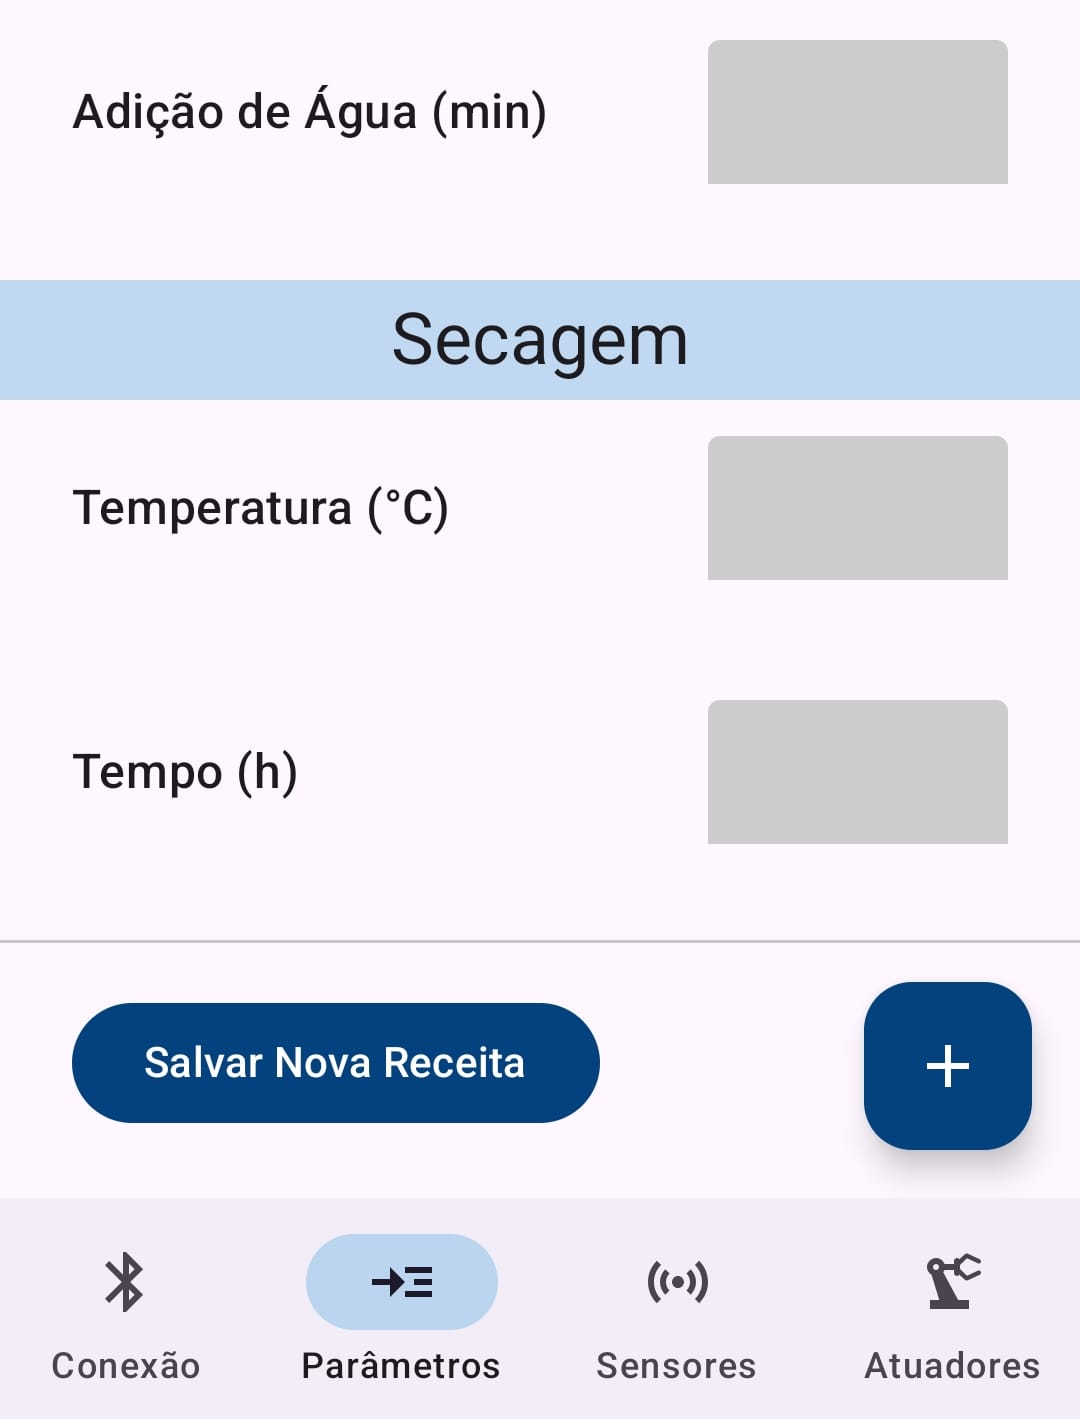
\includegraphics[width=0.32\textwidth]{save-recipe.jpeg}}
    \hfill
    \subfloat[Entrada de nome para salvamento de receita personalizada\label{fig:save-recipe-inputname}]{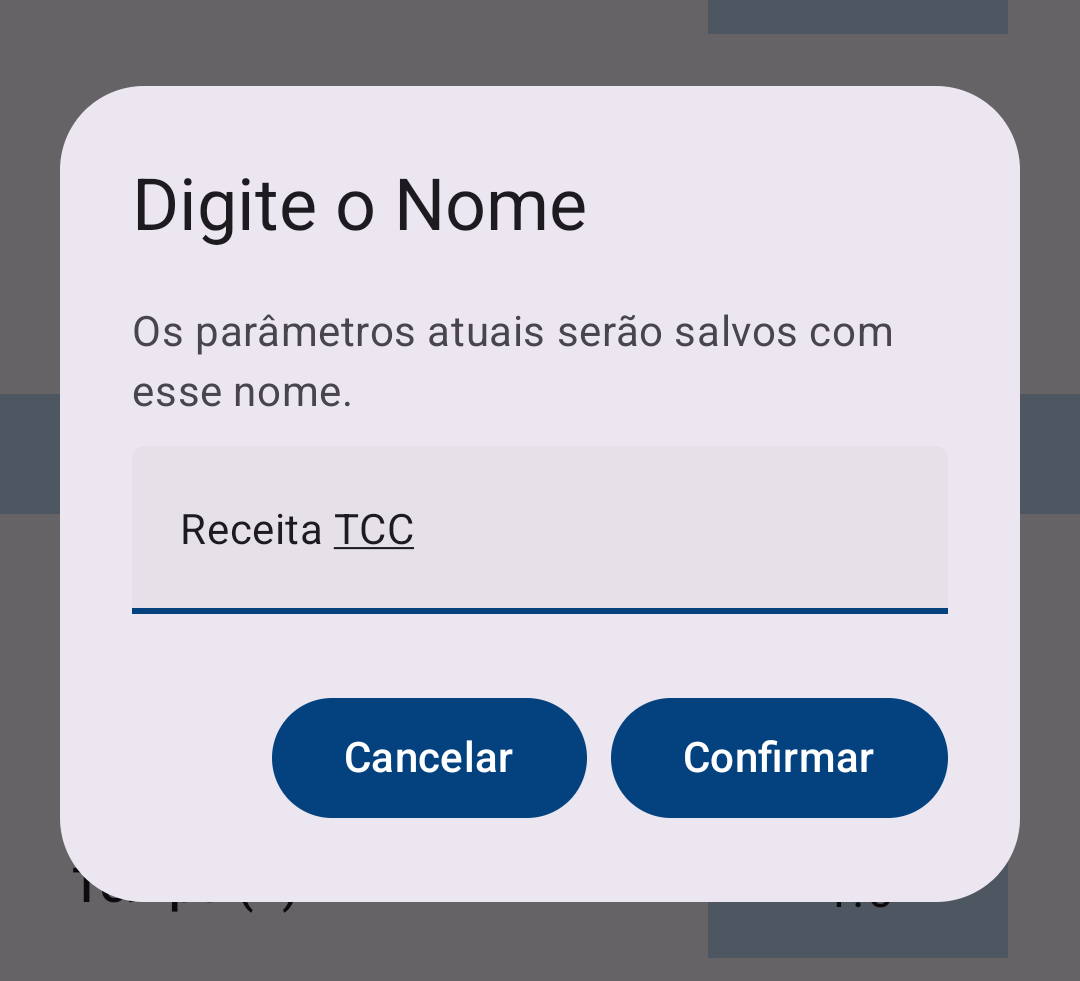
\includegraphics[width=0.32\textwidth]{save-recipe-inputname.png}}
    \hfill
    \subfloat[Seleção de receitas salvas\label{fig:select-recipe}]{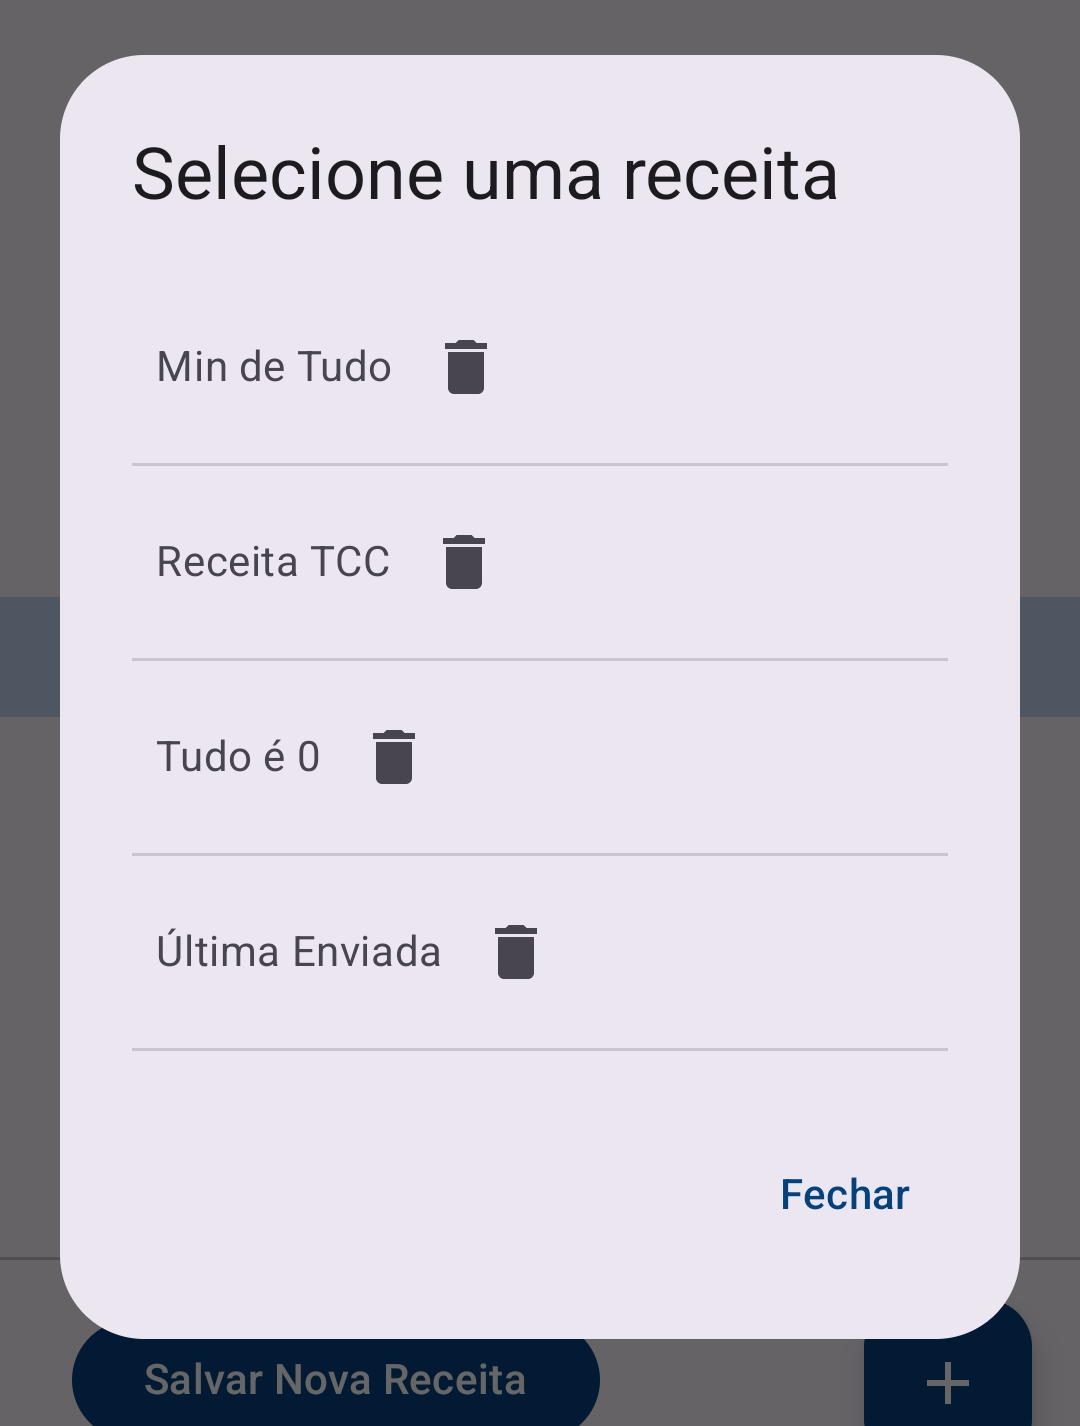
\includegraphics[width=0.32\textwidth]{select-recipe.png}}
    \hfill

    {\centering\footnotesize Fonte: Autoria própria.\par}

  \end{figure}

\subsection{Telas de Monitoramento: Sensores e Atuadores}\label{subsec:monitoramento}
As telas de sensores (\autoref{fig:sensors}) e atuadores (\autoref{fig:actuators}) cumprem função de monitoramento passivo, sem permitir interações diretas. A primeira exibe dados em tempo real de temperatura, umidade e concentração de CO$_2$, enquanto a segunda apresenta o estado operacional dos componentes físicos (válvulas, resistência, bomba de ar), com indicadores \textit{ON/OFF} gráficos. Ambas integram-se à \textit{BottomAppBar}, mantendo coerência na navegação e permitindo rápida alternância entre telas.

\begin{figure}[H]
    \caption{Interface de sensores}
    \label{fig:sensors}
    \centering
    \hfill
    \subfloat[Interface de sensores em modo desconectado\label{fig:sensores-off}]{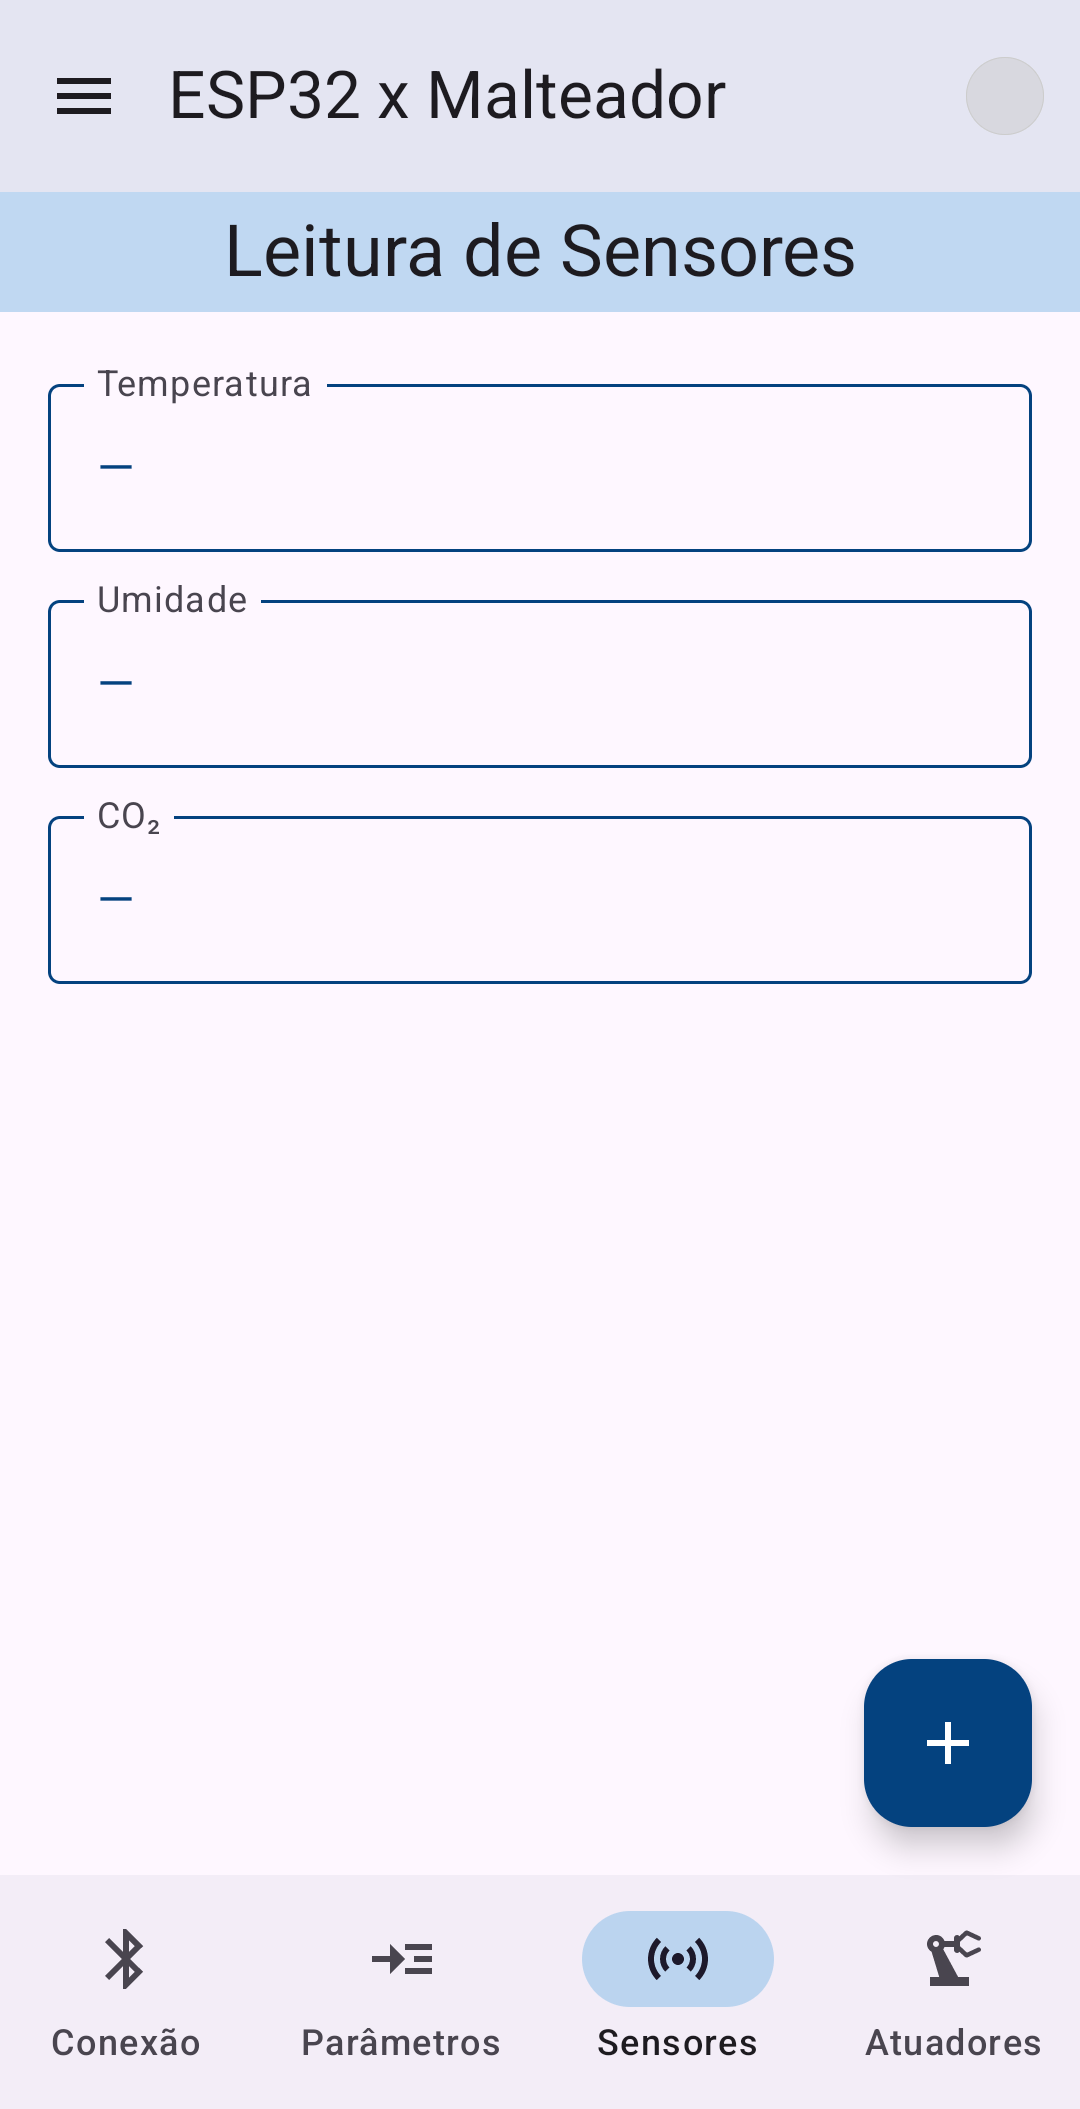
\includegraphics[width=0.3\textwidth]{sensores-off.png}}
    \hfill
    \subfloat[Interface de sensores em modo conectado\label{fig:sensores-on}]{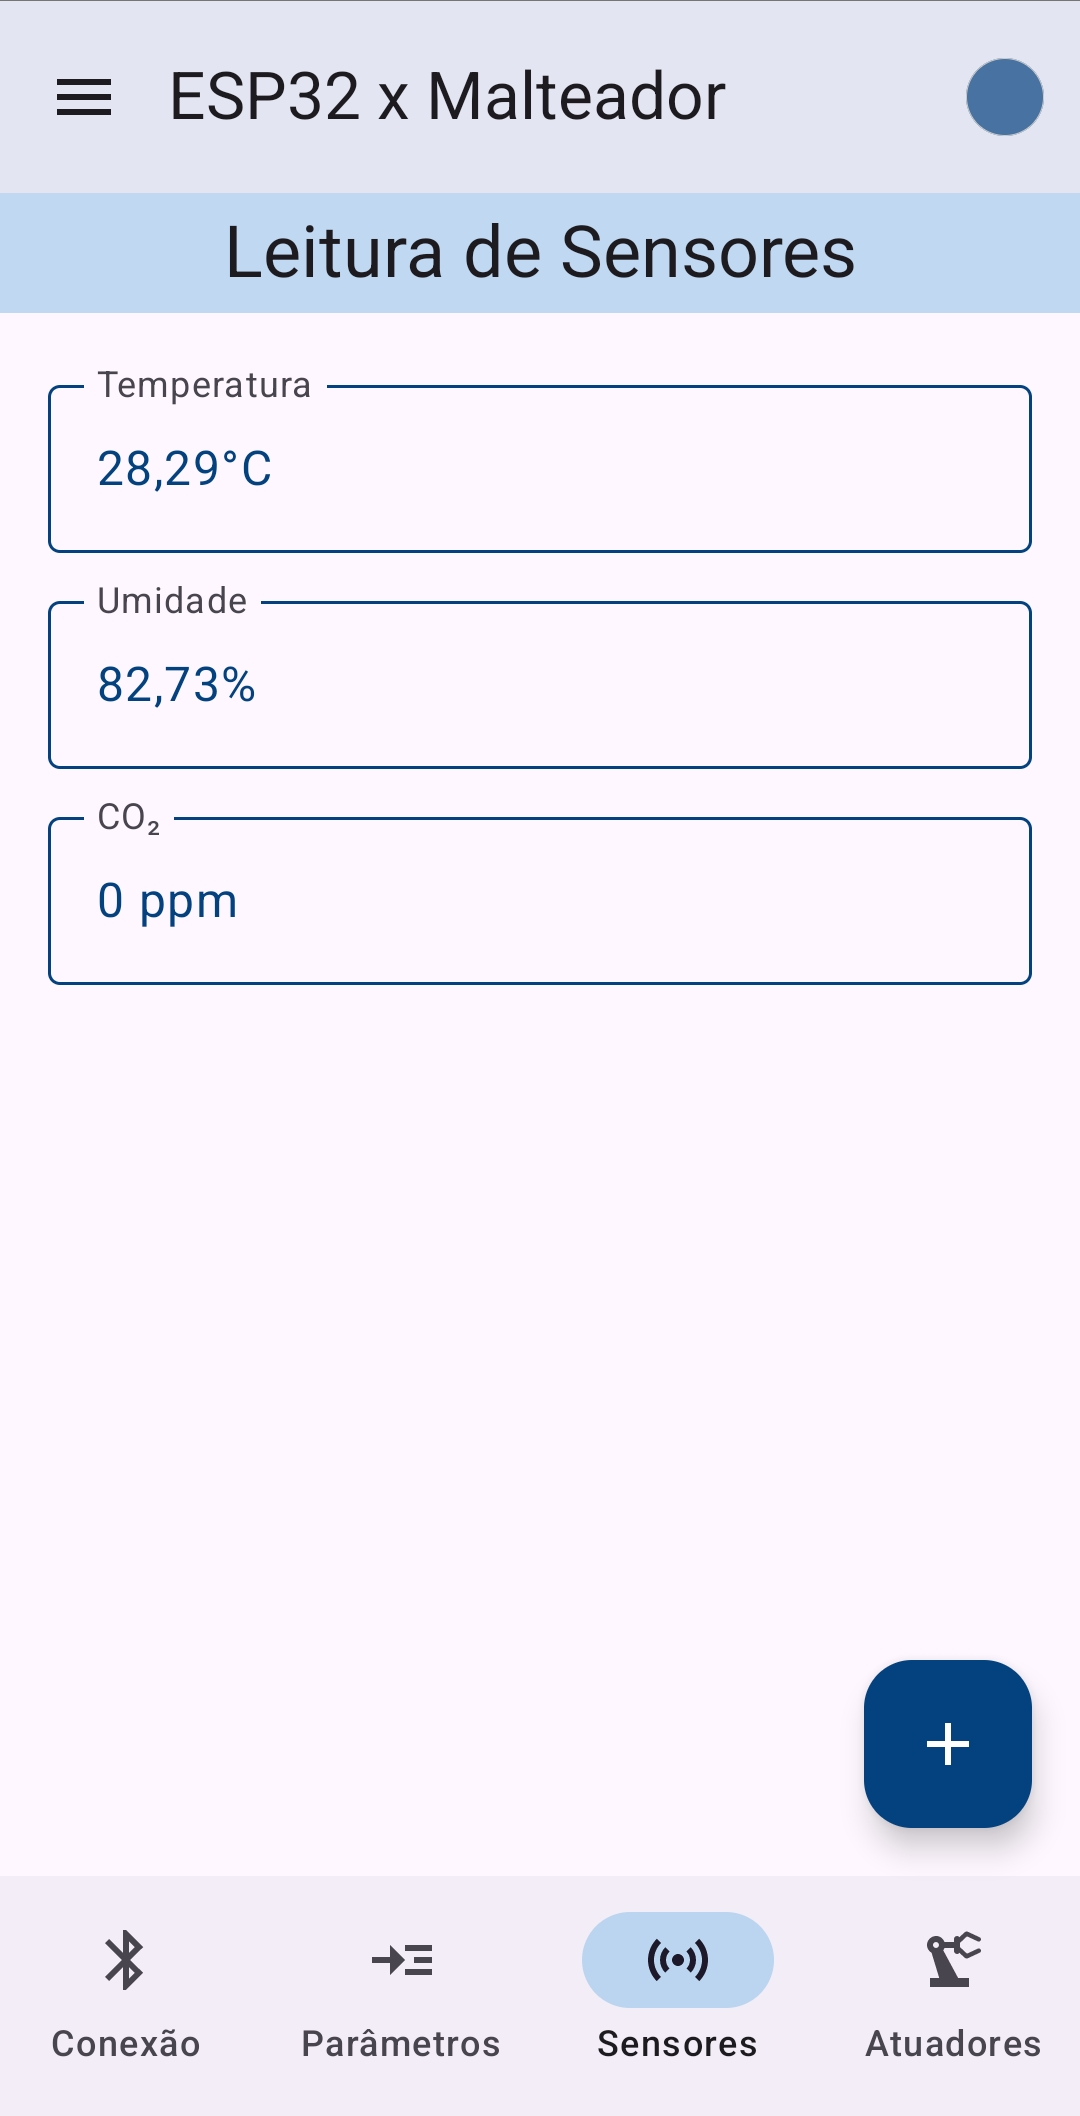
\includegraphics[width=0.3\textwidth]{sensores-on.png}}
    \hfill
    \hfill


    {\centering\footnotesize Fonte: Autoria própria.\par}

  \end{figure}

  \begin{figure}[H]
    \caption{Interface de atuadores.}
    \label{fig:actuators}
    \centering
    \hfill
    \subfloat[Estado dos atuadores em modo desconectado\label{fig:atuador-off}]{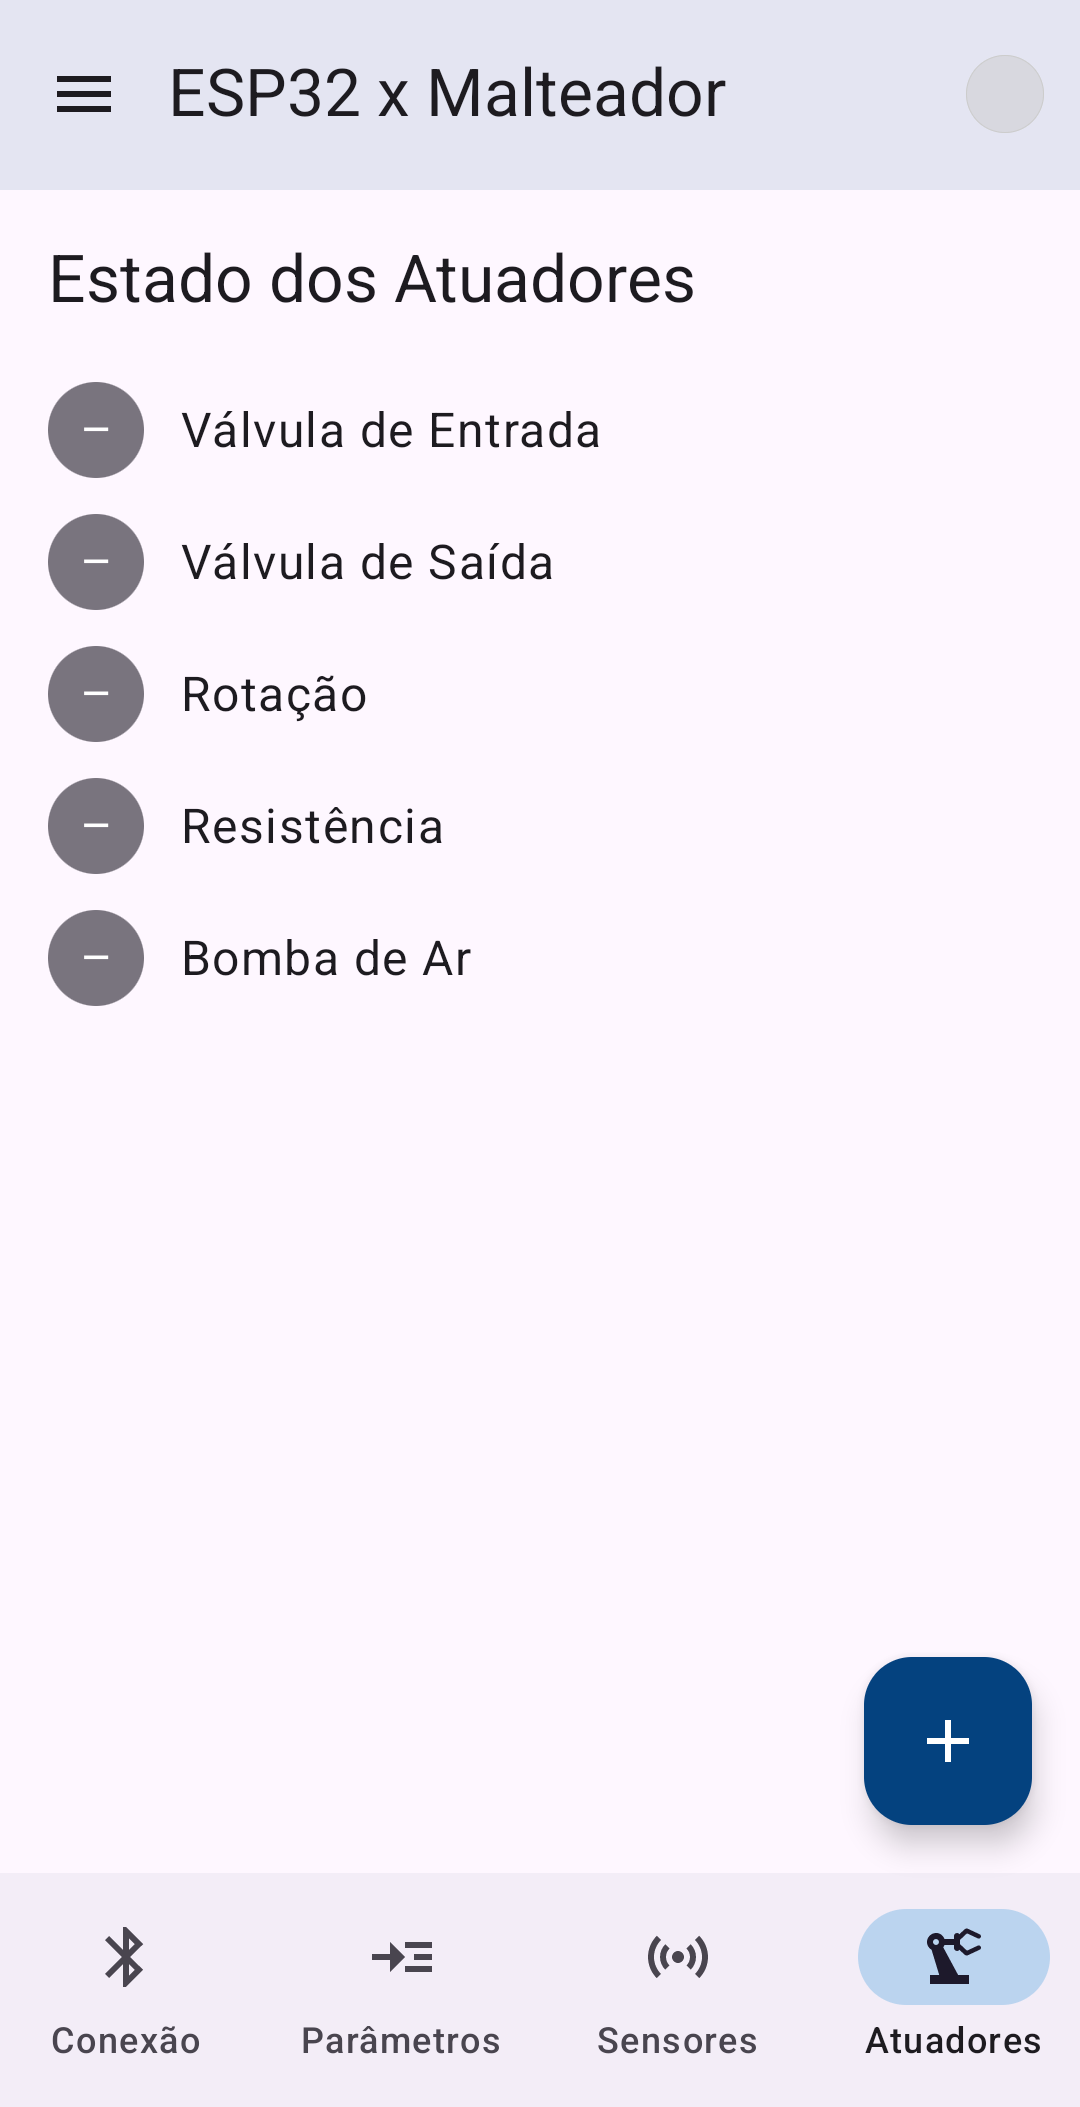
\includegraphics[width=0.3\textwidth]{atuador-off.png}}
    \hfill
    \subfloat[Interface de atuadores em modo conectado\label{fig:atuador-on}]{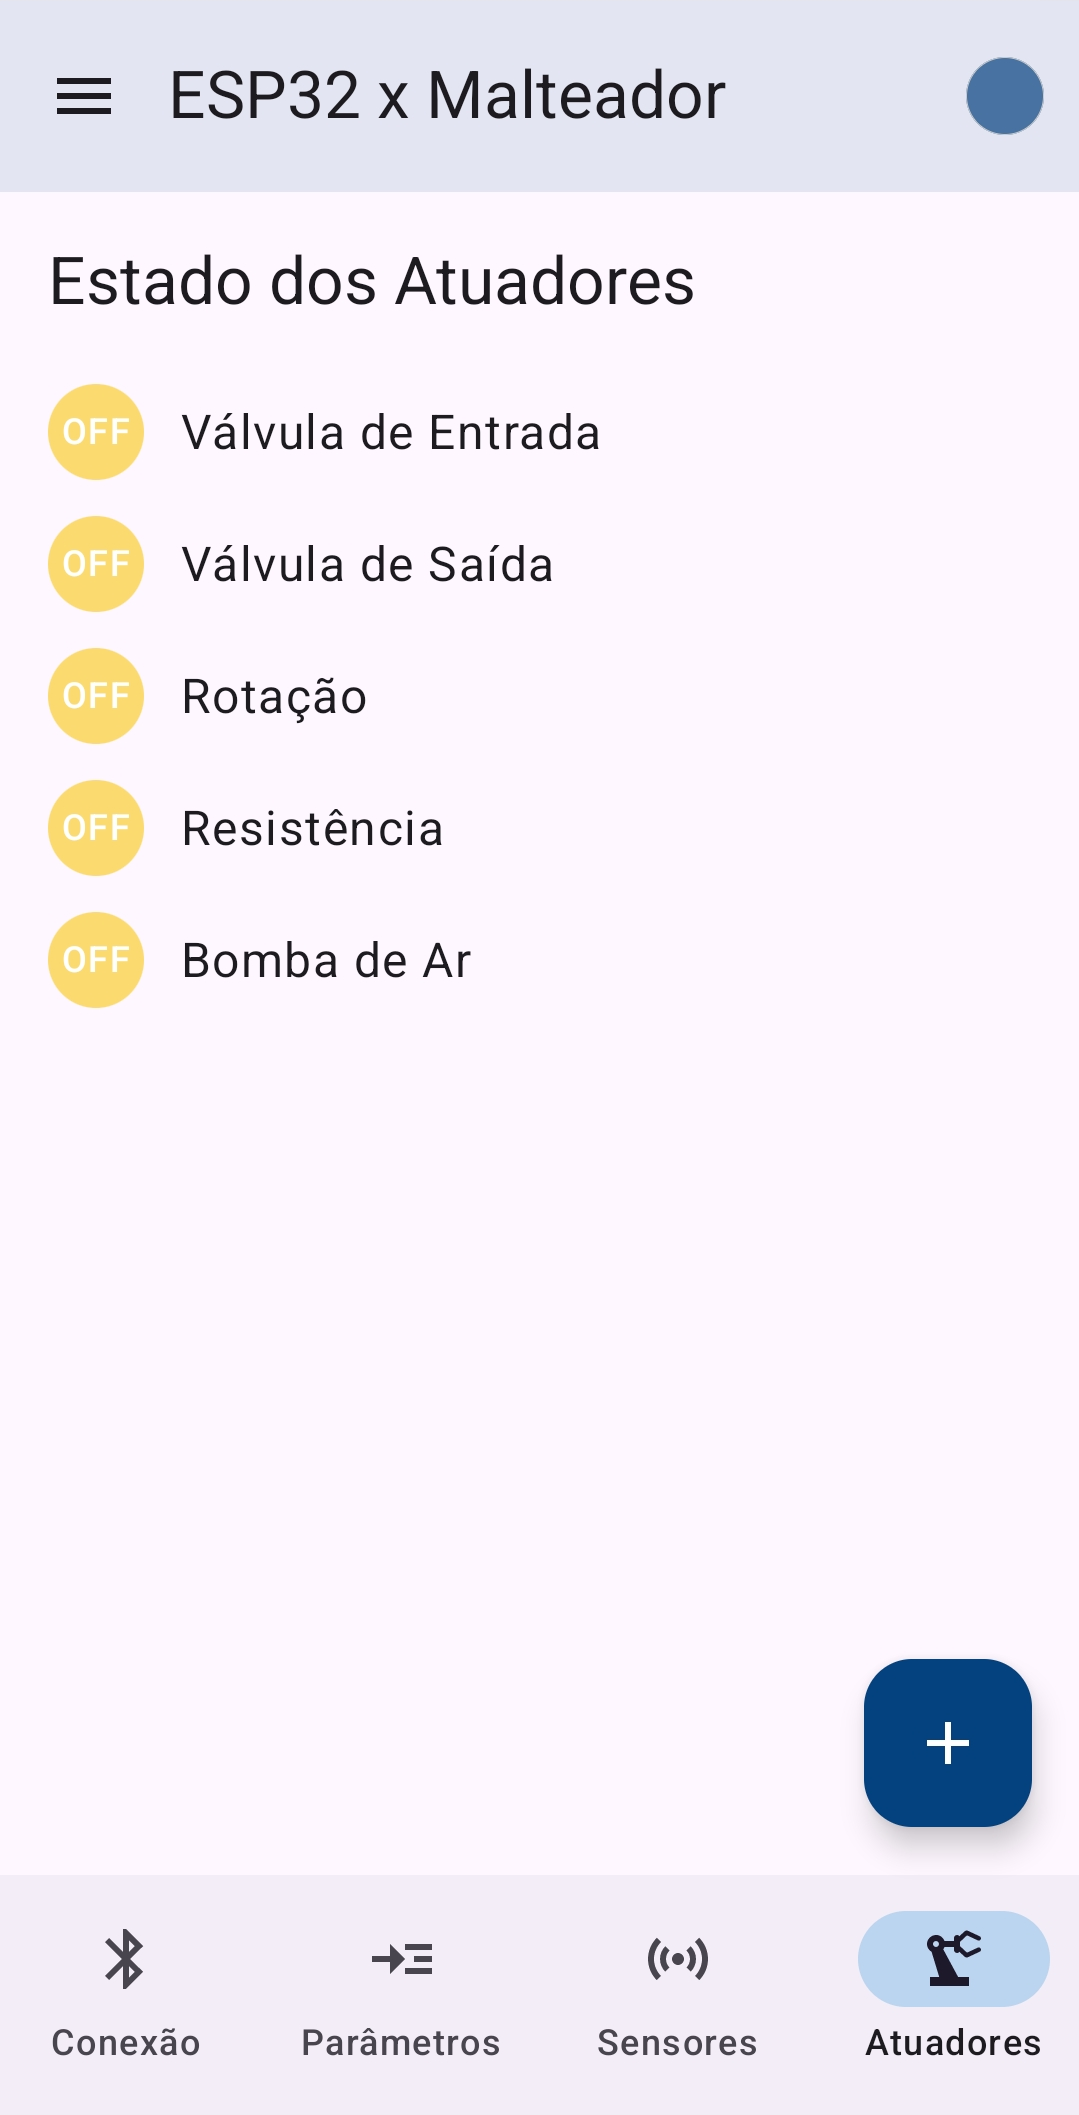
\includegraphics[width=0.3\textwidth]{atuador-on.png}}
    \hfill
    \hfill


    {\centering\footnotesize Fonte: Autoria própria.\par}

  \end{figure}

\section{Limitações e trabalhos futuros}

Embora a base dos \textit{softwares} estejam prontas, o presente trabalho apresenta limitações no que diz respeito à validação prática do sistema. O protótipo físico desenvolvido anteriormente, durante a IC, permanece incompleto em sua estrutura elétrica e nos componentes de automação, o que inviabilizou a realização de testes físicos com os controles implementados.
  
Como alternativa, recorreu-se à utilização do módulo de testes, o qual simulou os ciclos do processo com base na lógica implementada no \textit{firmware} (\texttt{v1.0-sim}) e no aplicativo (\texttt{v1.0}). A simulação permitiu validar o comportamento geral do sistema em condições normais de operação, com destaque para a lógica de controle assíncrona e a estabilidade da comunicação Bluetooth. A \autoref{fig:simulacaorodando} ilustra um momento da simulação em que o LED da porta 8 está aceso, indicando a ativação da saída responsável pela resistência, conforme a Tabela~\ref{tab:atuadores}.

\begin{figure}[H]
    \centering
    \caption{Quadro do vídeo da simulação realizada}
    \label{fig:simulacaorodando}
    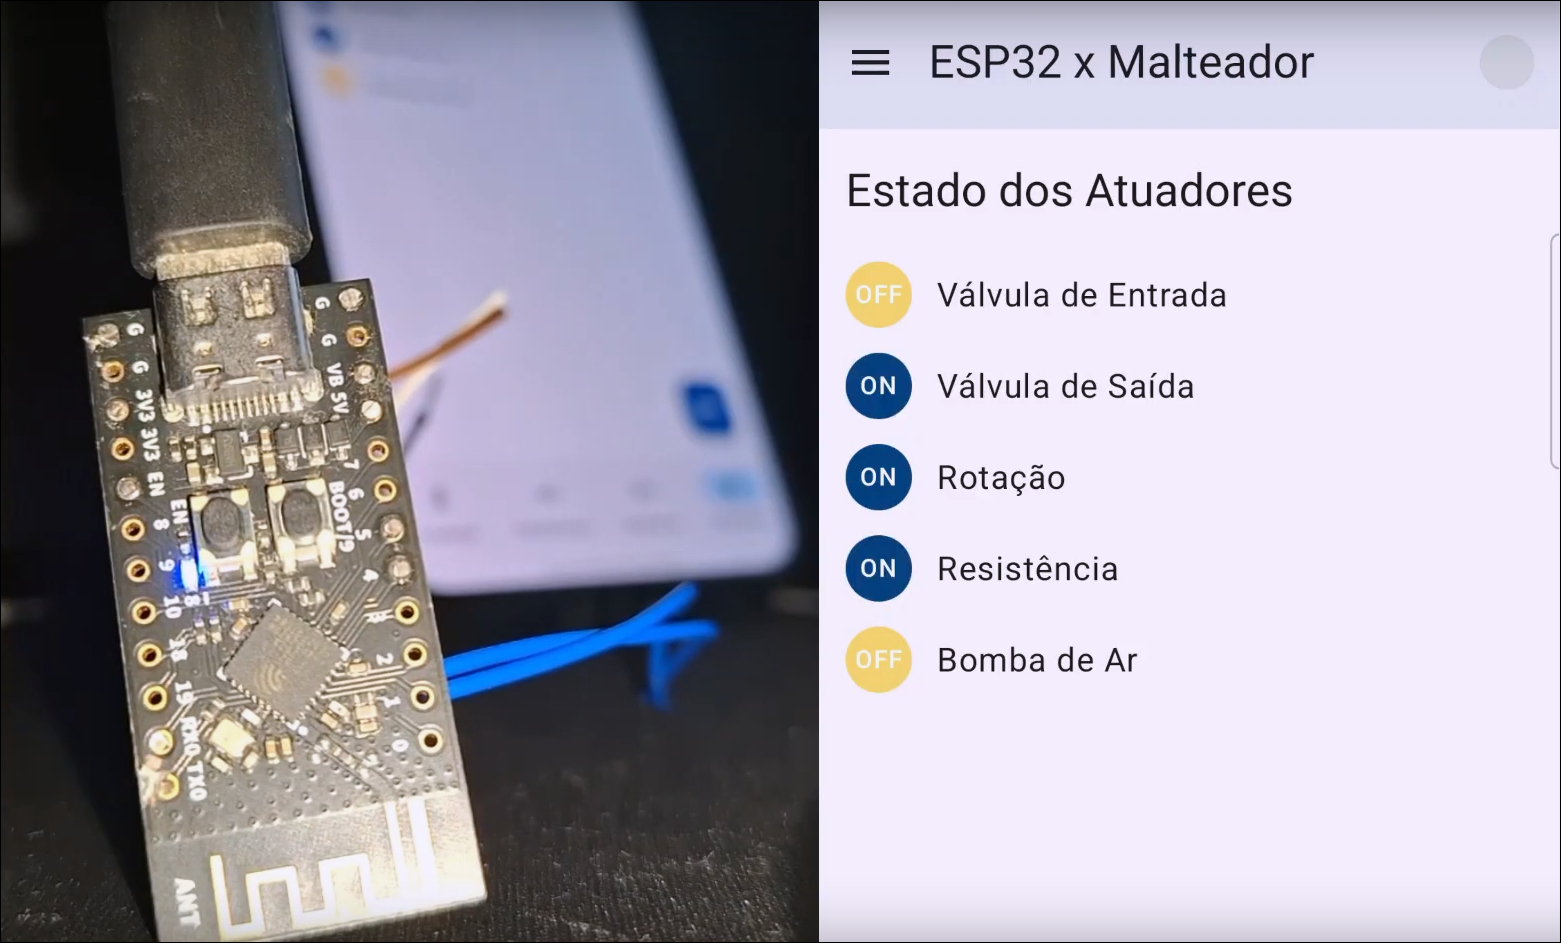
\includegraphics[width=0.9\textwidth]{simulacao-rodando.png}

    {\centering\footnotesize Fonte: Autoria própria.\par}
\end{figure}

Esta simulação não contou com leitura de sensores. Porém, em outros testes realizados, os sensores AH20 e ENS160 foram conectados ao sistema e realizaram leituras ambientais reais. Validando as lógicas associadas aos sensores.

Por fim, para trabalhos futuros, recomenda-se:
  
  \begin{itemize}
      \item Finalização do protótipo físico com sensores e atuadores totalmente integrados;
      \item Avaliação da eficiência do sistema em testes com diferentes perfis de malteação;
      \item Implementação de novos recursos, como adição de um programa de torrefação e exportação de dados históricos.
  \end{itemize}